
Esta sección presenta los resultados correspondientes a las etapas iniciales de preparación y diagnóstico de los datos, en coherencia con la metodología descrita previamente. En particular, se reportan los resultados del proceso de limpieza y filtrado, la identificación de datos faltantes y analisis univariados, anañlisis de cruces de variables, implemnation de PCA, algoritmos de agrupación y modelo \emph{pogit}.

%--------------------------------------------------
\section{Limpieza, filtrado y reglas explícitas}
    El conjunto de datos original contenía un total de 106{,}254 registros a nivel de línea de factura. Tras restringir el análisis a clientes empresariales y aplicar las reglas explícitas de limpieza y filtrado definidas en la sección metodológica anterior, el tamaño de la base de datos se redujo de manera sustancial.

    En primer lugar, se eliminaron las observaciones asociadas a devoluciones, notas crédito y anulaciones, identificadas mediante la variable \texttt{TIPO\_FACT}. Posteriormente, se abordó la presencia de registros duplicados a partir de la combinación \texttt{COD\_CLIENTE}--\texttt{NUM\_FACT}--\texttt{LINEA}, consolidando aquellos casos que correspondían a fragmentaciones de un mismo registro transaccional y eliminando los duplicados exactos.
    
    Adicionalmente, se excluyeron las filas que no contaban con un identificador válido de cliente, así como aquellas observaciones con fechas inválidas o ubicadas fuera del rango temporal definido para el estudio. Estas exclusiones se realizaron de manera sistemática y siguiendo criterios uniformes para toda la base de datos.
    
    Como resultado de este proceso, el conjunto final queda conformado por 27{,}850 registros a nivel de línea de factura. Esta reducción refleja la aplicación de reglas de depuración estructural orientadas a garantizar la consistencia interna y la trazabilidad de la información, y no responde a criterios ad hoc ni a transformaciones estadísticas destinadas a influir en los resultados del modelamiento.

%--------------------------------------------------
\section{Identificación de datos faltantes}
    Una vez completado el proceso de limpieza y filtrado de los registros transaccionales, se evaluó de manera sistemática la presencia de valores faltantes en cada una de las variables consideradas para el análisis. Este diagnóstico se realiza sobre la base final de clientes empresariales y permitió verificar la necesidad —o no— de aplicar procedimientos de imputación.

    Los resultados indican que no se identificaron valores faltantes en ninguna de las variables incluidas, tanto transaccionales como de perfilamiento del cliente, ni en las variables monetarias utilizadas para la construcción de la variable respuesta del modelo \emph{pogit}. Este resultado confirma la integridad estructural de la base de datos resultante tras las etapas previas de depuración.
    
    La ausencia total de valores faltantes simplifica el pipeline de preprocesamiento al eliminar la necesidad de introducir supuestos adicionales mediante técnicas de imputación. Desde una perspectiva estadística, esto reduce el riesgo de sesgos inducidos y evita un aumento innecesario en la varianza de las estimaciones, fortaleciendo la validez interna de los análisis posteriores y de la estimación del modelo \emph{pogit}.


%--------------------------------------------------
\section{Ventanas temporales y partición de los datos en conjuntos de entrenamiento y prueba}

    La aplicación del diseño temporal y muestral definido en la metodología dio lugar a la consolidación de una cohorte de análisis compuesta por \(N = 310\) clientes empresariales que realizaron al menos una compra a la empresa focal durante la ventana de características \(T_{1}\).

    Sobre esta cohorte se efectuó una partición aleatoria a nivel de cliente, dando lugar a un conjunto de entrenamiento conformado por 217 clientes (70\% de la muestra) y un conjunto de prueba integrado por 93 clientes (30\%). Esta asignación se mantuvo fija a lo largo de todas las etapas posteriores del análisis.
    
    La separación temporal estricta entre \(T_{1}\) y \(T_{2}\), junto con la partición a nivel de cliente, asegura que las variables predictoras y la variable respuesta se construyan sin solapamiento de información. En consecuencia, las estimaciones obtenidas para la \emph{Share--of--Wallet} y el \emph{Size--of--Wallet} en el conjunto de prueba corresponden a inferencias genuinamente fuera de muestra, consistentes con el diseño metodológico propuesto.
        
%--------------------------------------------------
\section{Construcción de variables predictoras}

    La aplicación del procedimiento de construcción de variables descrito en la metodología dio lugar a una base consolidada a nivel de cliente que integra información transaccional y de perfilamiento observada durante la ventana de características \(T_1\). Esta base constituye el insumo principal para las etapas posteriores de reducción de dimensionalidad, estimación del modelo \emph{pogit} y análisis exploratorio.

    \begin{table}[H]
    \centering
    \caption{Variables predictoras construidas a nivel de cliente a partir de la ventana de características \(T_1\).}
    \label{tab:base_empresas}
    \resizebox{\textwidth}{!}{%
    \begin{tabular}{lll}
    \hline
    \textbf{Variable} & \textbf{Tipo de variable} & \textbf{Descripción / categoría de referencia} \\
    \hline
    \multicolumn{3}{l}{\textbf{Identificador}} \\
    Cod cliente & Identificador (factor) & Identificador único del cliente. \\
    \hline
    \multicolumn{3}{l}{\textbf{Variables cuantitativas}} \\
    Recency & Cuantitativa continua & Días desde la última compra al 31/12/2023. \\
    Frequency & Cuantitativa discreta & Número total de compras del cliente. \\
    Monetary & Cuantitativa continua & Valor total gastado por el cliente. \\
    Valor bruto & Cuantitativa continua & Suma del valor bruto de las compras. \\
    Valor neto & Cuantitativa continua & Suma del valor neto de las compras. \\
    Cantidad & Cuantitativa discreta & Total de unidades adquiridas. \\
    Costo total & Cuantitativa continua & Costo total asociado a las compras. \\
    Utilidad bruta & Cuantitativa continua & Utilidad bruta total generada. \\
    SKUs distintos & Cuantitativa discreta & Número de referencias (SKU) distintas. \\
    Descuento (mediana) & Cuantitativa continua & Mediana del descuento aplicado (\texttt{desc1}). \\
    \hline
    \multicolumn{3}{l}{\textbf{Variables cualitativas (codificadas como dummies)}} \\
    País & Cualitativa nominal & País modal (ref.: Colombia). \\
    Departamento & Cualitativa nominal & Departamento modal (ref.: Antioquia). \\
    Ciudad & Cualitativa nominal & Ciudad modal (ref.: Ciudad de México). \\
    Tipo de empresa & Cualitativa nominal & Tipo modal (ref.: Editorial). \\
    Tipo de factura & Cualitativa nominal & Tipo de factura más frecuente. \\
    Tipo & Cualitativa nominal & Tipo de producto u operación modal. \\
    Grupo & Cualitativa nominal & Grupo de producto modal. \\
    Nombre de clase & Cualitativa nominal & Clase de producto modal. \\
    Clase 2 & Cualitativa nominal & Subclase de producto modal. \\
    Tamaño & Cualitativa ordinal & Tamaño modal del producto. \\
    SKU (Nom ISBN) & Cualitativa nominal & SKU o ISBN modal. \\
    Condición & Cualitativa nominal & Condición comercial modal (ref.: Anticipado). \\
    Categoría & Cualitativa nominal & Categoría de producto modal (ref.: Fina). \\
    Audiencia & Cualitativa nominal & Audiencia modal (ref.: Tipo 1). \\
    Zona & Cualitativa nominal & Zona geográfica modal (ref.: A). \\
    Mes & Cualitativa nominal & Mes modal de compra (ref.: Abril). \\
    \hline
    \end{tabular}
    }
    \end{table}

    El conjunto resultante incluye variables cuantitativas asociadas a la intensidad, recurrencia y magnitud económica de la relación comercial con la empresa focal, así como variables cualitativas que capturan características estructurales y contextuales del cliente empresarial. Las variables categóricas fueron transformadas en representaciones numéricas mediante variables indicadoras, omitiendo una categoría de referencia por factor, lo que garantiza la identificabilidad de los parámetros en los modelos posteriores.
    
    La Tabla~\ref{tab:base_empresas} presenta el universo de variables predictoras construidas a nivel de cliente a partir de la información observada durante \(T_1\). Este conjunto de variables sirve como base para la definición posterior de las matrices de diseño \(\mathbf{W}\) (mecanismo de asignación) y \(\mathbf{V}\) (mecanismo de intensidad) del modelo \emph{pogit}. 
    
    Es importante destacar que la construcción de esta base no implica la inclusión simultánea de todas las variables en una única especificación del modelo. Como se muestra en secciones posteriores, distintas selecciones y transformaciones de este conjunto inicial influyen en la estabilidad, parsimonia e interpretabilidad de las estimaciones, motivando el uso de estrategias de reducción de dimensionalidad y especificaciones alternativas del modelo.

%--------------------------------------------------
\section{Construcción de la variable respuesta}

    La variable respuesta utilizada en el modelo \emph{pogit} corresponde a \(y_i\), definida en la metodología como un \emph{proxy discretizado y normalizado} del gasto del cliente en la empresa focal durante la ventana de evaluación \(T_2\). Como se estableció previamente, \(y_i\) no representa un monto monetario ni un conteo físico de transacciones, sino una cantidad artificial expresada en una escala discreta inducida por la constante de discretización \(c\), estimada exclusivamente a partir del conjunto de entrenamiento.
    
    En la aplicación empírica considerada, la constante de discretización toma el valor
    \[
    c = 93{,}974{,}801 \text{ pesos colombianos}.
    \]
    Este escalamiento implica que tanto la variable observada \(y_i\) como la variable latente de intensidad \(n_i\) se expresan en una misma escala normalizada, distinta de la escala monetaria original. En consecuencia, los valores de \(y_i\) deben interpretarse únicamente en términos relativos, como órdenes de magnitud discretizados del gasto del cliente en la empresa focal, y no como valores económicos directamente observables.
    
    La distribución empírica de \(y_i\), calculada sobre el conjunto de prueba utilizando la constante \(c\) estimada en el conjunto de entrenamiento, muestra una fuerte concentración en valores bajos. En particular, la variable toma valores únicamente en el conjunto \(\{0,1,2\}\), con una mayoría de clientes empresariales ubicados en \(y_i = 0\). Este patrón refleja directamente el procedimiento de discretización aplicado al gasto monetario y es coherente con la estructura altamente asimétrica característica de datos B2B, donde una fracción reducida de clientes concentra niveles elevados de actividad económica.
    
    Dado el carácter discreto y acotado de la variable respuesta, la heterogeneidad transversal entre clientes no se manifiesta a través de grandes diferencias en magnitud absoluta, sino mediante la probabilidad de ocupar niveles discretos más altos en la escala de \(y_i\). Esta característica es plenamente consistente con el marco del modelo \emph{pogit}, en el cual la información relevante para la inferencia sobre la \emph{Share--of--Wallet} y el \emph{Size--of--Wallet} se extrae de la relación entre la variable observada \(y_i\) y el volumen latente total \(n_i\), ambos definidos en la misma escala discretizada.
    
    La Tabla~\ref{tab:resumen_y} presenta la distribución empírica observada de la variable respuesta en la ventana de evaluación \(T_2\).
    
    \begin{table}[H]
    \centering
    \caption{Distribución empírica de la variable respuesta \(y_i\) en la ventana \(T_2\).}
    \label{tab:resumen_y}
    \begin{tabular}{ccc}
    \hline
    Valor de \(y_i\) & Frecuencia & Porcentaje \\
    \hline
    0 & 198 & 91.24\% \\
    1 & 10  & 4.61\% \\
    2 & 9   & 4.15\% \\
    \hline
    Total & 217 & 100\% \\
    \hline
    \end{tabular}
    \end{table}
    
    Es importante enfatizar que esta distribución no constituye una limitación empírica del análisis, sino una consecuencia natural del escalamiento adoptado y del uso de un modelo de conteos latentes para compatibilizar información monetaria continua con un marco Poisson--Binomial. En este contexto, la variable \(y_i\) actúa como un ancla observacional que permite inferir simultáneamente la intensidad latente total de consumo en la categoría y la fracción de dicha intensidad asignada a la empresa focal.
    
%--------------------------------------------------
\section{Análisis exploratorio}
    En esta sección se presentan los resultados del análisis exploratorio de las variables predictoras construidas a partir de la ventana \(T_1\). El análisis tiene un carácter estrictamente descriptivo y diagnóstico, y su propósito es caracterizar la estructura de los datos, identificar patrones relevantes y documentar la heterogeneidad transversal entre clientes empresariales, sin introducir aún transformaciones ni criterios formales de selección.
    
    \subsection{Análisis univariado de variables cuantitativas predictoras}
    
    La Tabla~\ref{fig:tablarecency} resume las principales estadísticas descriptivas de las variables cuantitativas utilizadas como predictores del modelo \emph{pogit}. Los histogramas y diagramas de caja correspondientes se presentan en el Apéndice~\ref{sec:variablescuantitativas} como apoyo visual para la interpretación de las distribuciones observadas.
    
    \begin{table}[H]
    \centering
    \caption{Resumen estadístico de las variables cuantitativas predictoras}
    \label{fig:tablarecency}
    \resizebox{\textwidth}{!}{%
    \begin{tabular}{lcccccccc}
    \hline
    \textbf{Variable} & \textbf{Media} & \textbf{Mín.} & \textbf{Q1} & \textbf{Mediana} & \textbf{Q3} & \textbf{Máx.} & \textbf{CV (\%)} & \textbf{Outliers (\%)} \\
    \hline
    Recency & 235.4 & 9 & 79 & 207.5 & 304 & 668 & 79.3 & 4.2 \\
    Frequency & 65.4 & 1 & 2 & 4 & 32.8 & 3,551 & 360.0 & 18.4 \\
    Monetary & 98,829,834 & 2,526 & 943,190 & 2,510,924 & 14,150,826 & 5,617,572,866 & 438.0 & 17.0 \\
    Valor neto & 8,555,464 & 862 & 16,200 & 43,800 & 670,110 & 109,403,195 & 349.0 & 20.0 \\
    Valor bruto & 4,401,277 & 548 & 20,000 & 65,000 & 2,167,279 & 206,973,510 & 353.0 & 16.1 \\
    Costo total & 60,957,738 & 1,742 & 380,071 & 1,230,277 & 6,609,727 & 3,926,358,043 & 466.0 & 16.0 \\
    Cantidad & 6,075 & 6 & 65 & 180 & 790 & 209,131 & 377.0 & 16.0 \\
    Descuento & 21.3 & 0 & 10.0 & 19.0 & 31.6 & 60.0 & 67.0 & 0.0 \\
    SKUs distintos & 25.5 & 1 & 1 & 2 & 22 & 321 & 187.0 & 17.1 \\
    \hline
    \end{tabular}}
    \end{table}
    
    Del análisis univariado se tiene:
    
    \begin{itemize}
    \item Todas las variables cuantitativas presentan distribuciones marcadamente asimétricas a la derecha, con colas largas y presencia significativa de valores extremos (ver Apéndice~\ref{sec:variablescuantitativas}). Este patrón es característico de datos transaccionales en contextos B2B y sugiere una elevada concentración del volumen de actividad en un subconjunto reducido de clientes.
    
    \item El coeficiente de variación supera ampliamente el 100\% en la mayoría de las variables monetarias y de volumen, alcanzando valores cercanos o superiores al 400\%. Esto evidencia una heterogeneidad extrema en la escala de las covariables, que debe ser considerada cuidadosamente en las etapas posteriores del análisis.
    
    \item La proporción de observaciones atípicas se sitúa entre el 16\% y el 20\% para la mayoría de las variables económicas y de cantidad, lo que indica la presencia sistemática de valores extremos que podrían afectar la estabilidad numérica de los modelos si no se tratan adecuadamente.
    
    \item En términos de recencia, el 75\% de los clientes realizó su última compra en un periodo igual o inferior a 304 días, mientras que la mediana de 208 días sugiere la coexistencia de clientes relativamente activos con otros que presentan lapsos prolongados de inactividad.
    
    \item La frecuencia de compra muestra una distribución altamente concentrada en valores bajos, con una mediana de 4 transacciones, en contraste con un número reducido de clientes que alcanza valores extremadamente altos. Este patrón anticipa la existencia de perfiles claramente diferenciados entre clientes ocasionales e intensivos.
    
    \item Las variables monetarias (\textit{Monetary}, \textit{Valor bruto}, \textit{Valor neto} y \textit{Costo total}) capturan distintas agregaciones económicas de la relación comercial y exhiben colas pesadas típicas de contextos B2B. En todos los casos, la mediana es sustancialmente inferior a la media, lo que confirma que unos pocos clientes de alto valor dominan el volumen total de ventas.
    
    \item La variable \textit{Cantidad} presenta un comportamiento análogo, con una mediana de 180 unidades y valores máximos que superan ampliamente las 200 mil unidades, reforzando la evidencia de heterogeneidad extrema en el volumen de compra.
    
    \item La variable \textit{Descuento} muestra una dispersión relativamente menor en comparación con el resto de las variables, con una mediana cercana al 19\%, aunque con presencia de algunos valores extremos.
    
    \item Finalmente, \textit{SKUs distintos} indica que la mayoría de los clientes adquiere un número reducido de referencias, mientras que existen casos extremos con portafolios amplios, lo que aporta información relevante sobre la diversidad de compra.
    \end{itemize}
    
    Estos resultados ponen de manifiesto la presencia de asimetrías severas, escalas muy dispares entre covariables y una proporción no despreciable de valores extremos. Estas características no se corrigen en esta etapa, pero motivan explícitamente la necesidad de aplicar procedimientos sistemáticos de tratamiento de valores extremos, estandarización y control de redundancias, tal como se describe en la sección de preprocesamiento.
    
    \subsection{Análisis descriptivo de variables categóricas}
    
    La Figura~\ref{figempresa} muestra que la mayor proporción del volumen transaccional corresponde a organizaciones religiosas, que concentran aproximadamente el 60\% del total. En segundo lugar se encuentran las editoriales (15\%) y las empresas comerciales (13.5\%). Esta distribución es coherente con la naturaleza del portafolio de la Empresa Distribuidora de Literatura Cristiana.
    
    Desde una perspectiva analítica, esta variable refleja heterogeneidad estructural entre clientes, dado que distintos tipos de empresa pueden diferir tanto en su intensidad total de consumo como en sus patrones de asignación del gasto hacia la empresa focal.

    La Figura~\ref{figmes} evidencia una marcada concentración del volumen de ventas en los meses de marzo y abril, consistente con eventos del calendario litúrgico. Este patrón se documenta como información contextual y no se incorpora directamente en el modelamiento para evitar fuga de información entre ventanas temporales.
    
    \begin{figure}[H]
    \centering
    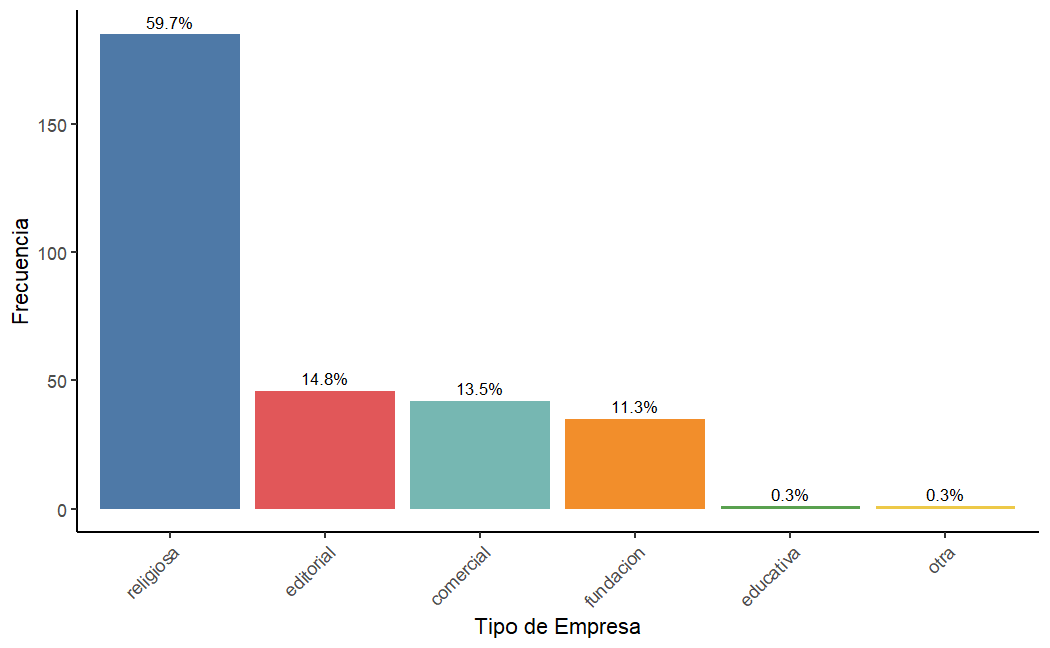
\includegraphics[width=0.8\textwidth]{figuras/Tipo_Empresa.png}
    \caption{\label{figempresa}Distribución del volumen transaccional por tipo de empresa.}
    \end{figure}
    
    \begin{figure}[H]
    \centering
    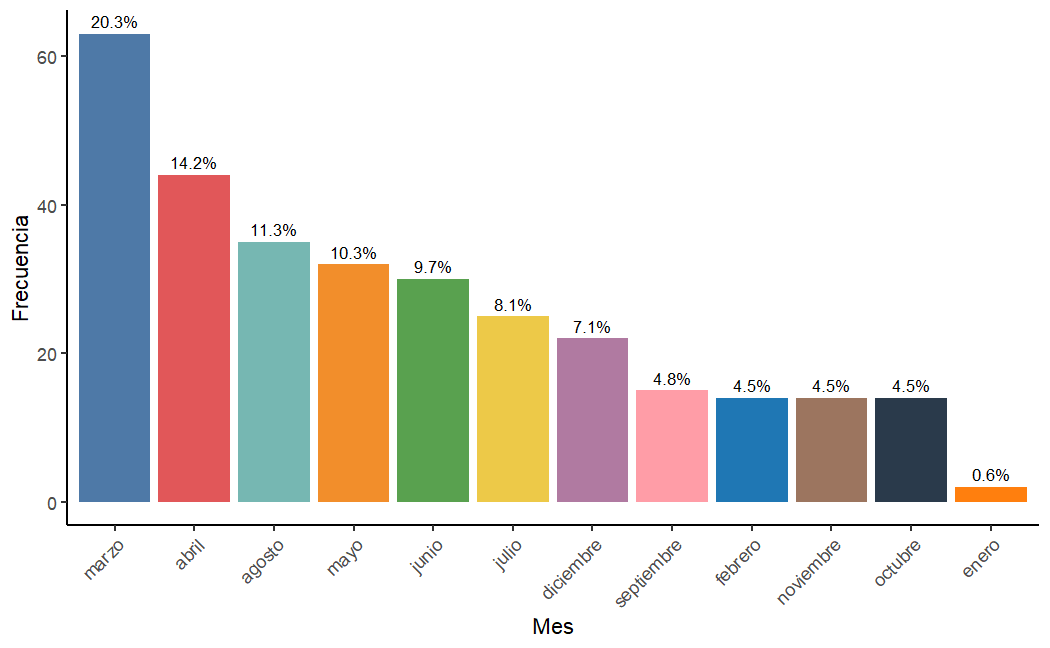
\includegraphics[width=0.8\textwidth]{figuras/Mes.png}
    \caption{\label{figmes}Distribución del volumen transaccional por mes.}
    \end{figure}
    
    En la Figura~\ref{figorigen} se observa que el 94\% del volumen de ventas proviene del mercado nacional. Aunque el segmento internacional es reducido, su identificación resulta relevante para caracterizar perfiles potencialmente diferenciados de asignación del gasto.

    La Figura~\ref{figciudad} muestra una fuerte concentración geográfica del volumen transaccional, con Bogotá como principal centro de demanda. Casos como Frontino, con una participación relevante pese a su menor tamaño relativo, sugieren la presencia de clientes institucionales de alto volumen.
    
    \begin{figure}[H]
    \centering
    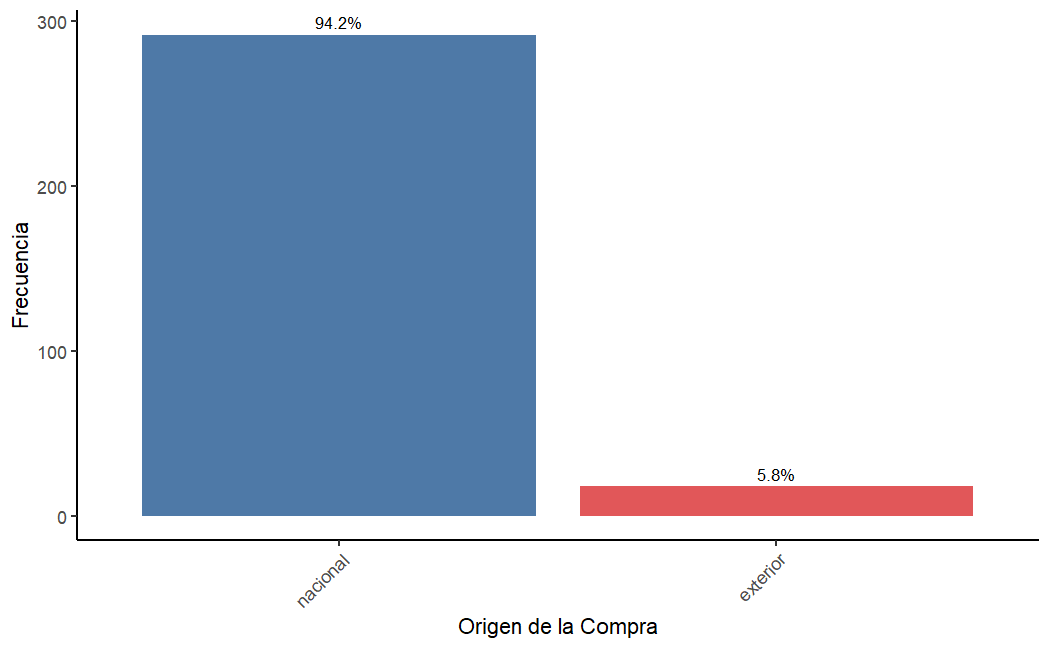
\includegraphics[width=0.8\textwidth]{figuras/Origen de Compra.png}
    \caption{\label{figorigen}Distribución del volumen transaccional según el origen de la compra.}
    \end{figure}
    
    \begin{figure}[H]
    \centering
    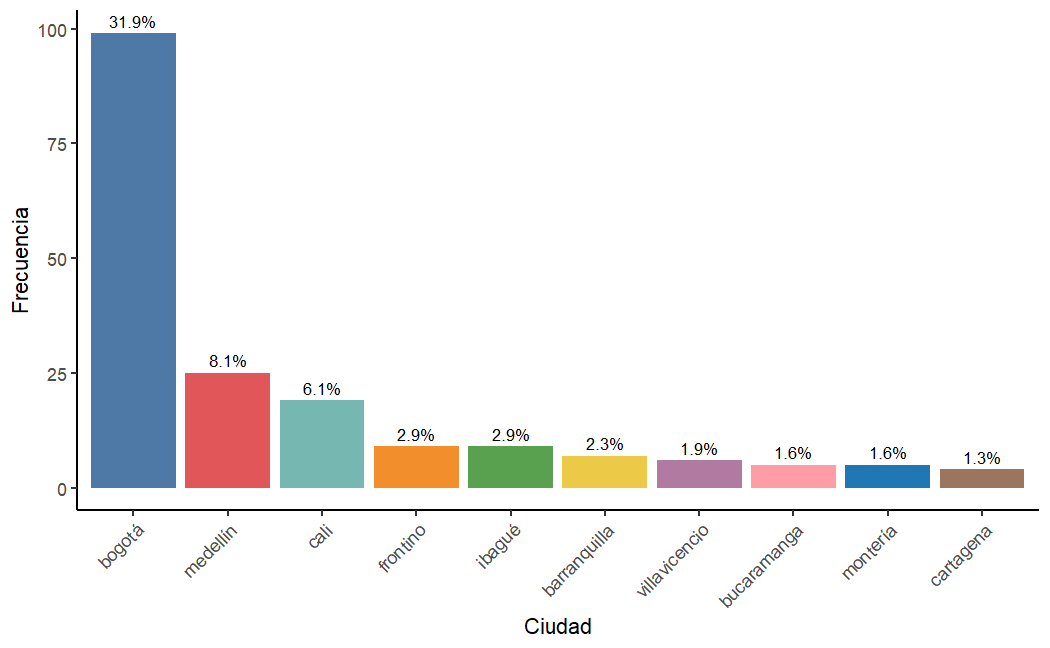
\includegraphics[width=0.8\textwidth]{figuras/Ciudad.png}
    \caption{\label{figciudad}Distribución del volumen transaccional por ciudad (Top 10).}
    \end{figure}
    
    En cuanto al portafolio de productos, la Figura~\ref{figtipoproducto} indica que cerca del 90\% del volumen corresponde a biblias, lo que implica una alta concentración en un único tipo de producto. En consecuencia, la diferenciación entre clientes se explica principalmente por variables de volumen, frecuencia, formato y diversidad de referencias, más que por la elección entre categorías.

    Finalmente, la Figura~\ref{figtamano} muestra una marcada preferencia por el formato Biblia Taco 60, que concentra cerca del 70\% del volumen total, lo que sugiere una estandarización importante en las decisiones de compra.

     El análisis exploratorio documenta la existencia de heterogeneidad estructural entre clientes, concentración del volumen transaccional y escalas altamente dispares entre covariables. Estos resultados se interpretan exclusivamente desde una perspectiva descriptiva y constituyen el insumo empírico para el diseño del preprocesamiento posterior, donde se implementan criterios formales para el tratamiento de valores extremos, la estandarización y el control de redundancias entre covariables.
    
    \begin{figure}[H]
    \centering
    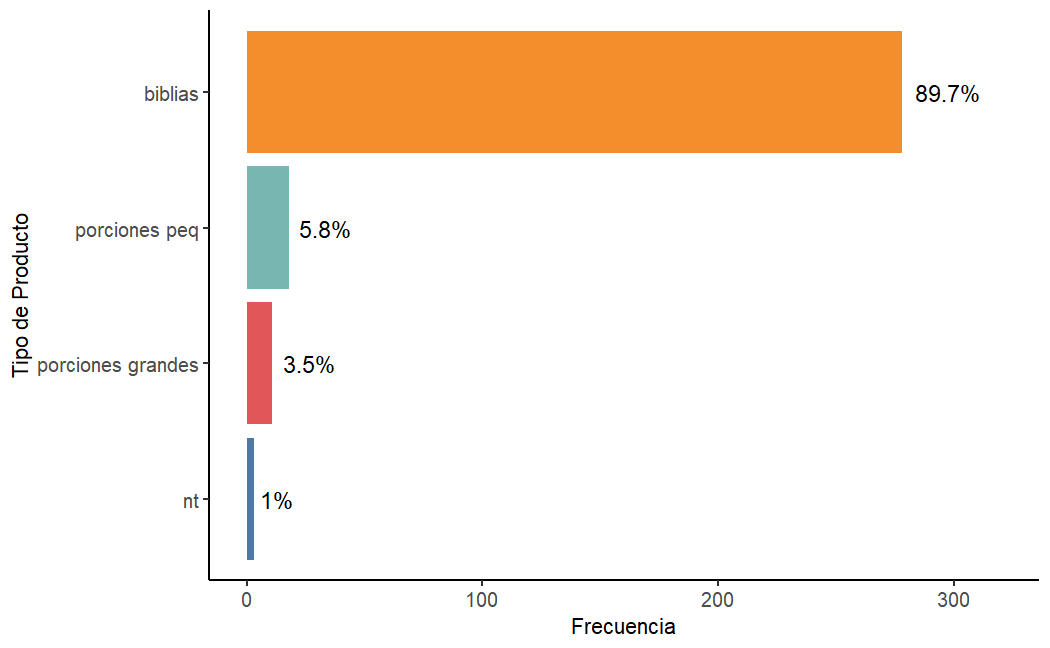
\includegraphics[width=0.8\textwidth]{figuras/Tipo Producto.png}
    \caption{\label{figtipoproducto}Distribución del volumen transaccional por tipo de producto.}
    \end{figure}
    
    \begin{figure}[H]
    \centering
    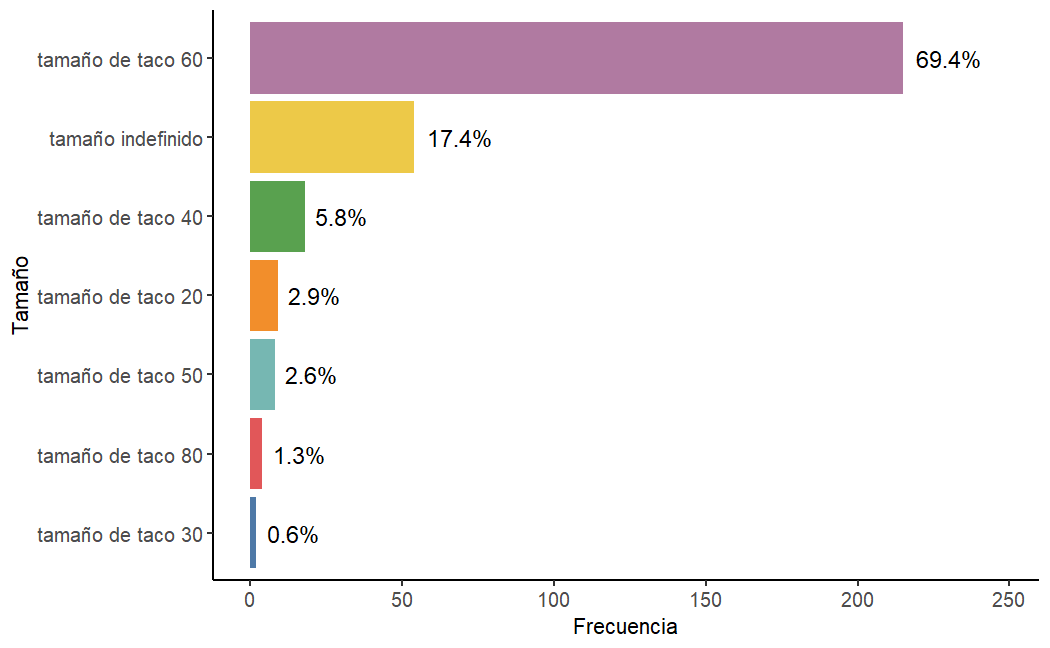
\includegraphics[width=0.8\textwidth]{figuras/Tamaño.png}
    \caption{\label{figtamano}Distribución del volumen transaccional por tamaño de producto.}
    \end{figure}
    
%--------------------------------------------------
\section{Preprocesamiento}

\subsubsection{Análisis de asociación entre variables cuantitativas}
        Con el fin de evaluar el grado de asociación entre las variables cuantitativas predictoras y detectar posibles redundancias, se calculó el coeficiente de correlación de Spearman. 
        
        La Tabla~\ref{tab:corr_cuantitativas} presenta las correlaciones de Spearman más altas observadas entre pares de variables cuantitativas. Con fines de depuración, se consideraron únicamente aquellas asociaciones cuyo coeficiente fue mayor o igual a 0.70 en valor absoluto, umbral comúnmente utilizado para identificar relaciones fuertes y potencialmente redundantes.

         De manera complementaria, se observa que la variable \textit{recency\_days} presenta correlaciones negativas moderadas a altas con el resto de variables cuantitativas (en el rango aproximado de -0.50 a -0.70), lo cual indica que mayores tiempos desde la última compra se asocian sistemáticamente con menores niveles de frecuencia, gasto y volumen adquirido. Dado que estas correlaciones negativas no superan el umbral absoluto adoptado para la identificación de asociaciones fuertes, no se incluyen en la tabla; no obstante, su patrón resulta plenamente consistente con la lógica del marco RFM.

        El análisis revela una fuerte asociación entre las variables \textit{Monetary}, \textit{Costo Total} y \textit{Utilidad Bruta}, con coeficientes de Spearman superiores a 0.95. Dado que estas variables capturan esencialmente la misma dimensión de escala económica del cliente, se decide conservar únicamente \textit{Monetary}, por su interpretación directa y su uso estándar en análisis RFM, y eliminar las restantes para reducir redundancia en el diseño del modelo.
        
        \begin{table}[H]
        \centering
        \caption{Correlaciones de Spearman más altas entre variables cuantitativas}
        \label{tab:corr_cuantitativas}
        \renewcommand{\arraystretch}{1.2}
        \resizebox{\textwidth}{!}{%
        \begin{tabular}{l l c @{~~~~} l l c}
        \hline
        \textbf{Variable 1} & \textbf{Variable 2} & \textbf{Spearman} &
        \textbf{Variable 1} & \textbf{Variable 2} & \textbf{Spearman} \\
        \hline
        Costo total & Monetary & 0.99 &
        Cantidad & Utilidad bruta & 0.85 \\
        
        Monetary & Utilidad bruta & 0.98 &
        Valor Bruto & Valor neto & 0.82 \\
        
        Costo total & Utilidad bruta & 0.96 &
        Utilidad bruta & Valor bruto & 0.79 \\
        
        Frequency & Skus distintos & 0.94 &
        Costo total & Frequency & 0.79 \\
        
        Frequency & Valor bruto & 0.93 &
        Monetary & Valor bruto & 0.78 \\
        
        Cantidad & Costo total & 0.90 &
        Frequency & Monetary & 0.78 \\
        
        Cantidad & Monetary & 0.89 &
        Costo total & Valor bruto & 0.78 \\
        
        Skus distintos & Valor bruto & 0.87 &
        Frequency & Utilidad bruta & 0.77 \\
        
        Descuentos & Valor neto & 0.76 &
        Frequency & Valor neto & 0.74 \\
        
        Costo total & Skus distintos & 0.71 &
        Cantidad & Frequency & 0.70 \\
        \hline
        \end{tabular}%
        }
        \end{table}

        Asimismo, se identifican correlaciones elevadas entre \textit{Frequency}, \textit{Skus Distintos} y \textit{Valor Bruto}. En este caso, se optó por conservar \textit{Frequency}, dado que representa de manera más directa la recurrencia del comportamiento de compra, y eliminar las otras variables altamente correlacionadas.
        
        Finalmente, dado que \textit{Valor Neto} presenta asociaciones fuertes con múltiples variables monetarias y de frecuencia, se decidió excluirla del conjunto de covariables para evitar solapamientos informativos.
        
        Como resultado de este proceso de depuración, se obtuvo el conjunto final de variables cuantitativas que se utilizarán en la construcción de la matriz de diseño del modelo \emph{pogit}, el cual se resume en la Tabla~\ref{tab:depuracion_cuantitativas}.
        
        \begin{table}[H]
        \centering
        \caption{Variables cuantitativas seleccionadas y eliminadas tras el análisis de asociación}
        \label{tab:depuracion_cuantitativas}
        \renewcommand{\arraystretch}{1.2}
        \begin{tabular}{p{7cm} p{7cm}}
        \hline
        \textbf{Permanecen en el modelo} & \textbf{Eliminadas del modelo} \\
        \hline
        \textit{monetary}, \textit{frequency} 
        & \textit{costo\_total}, \textit{utilidad\_bruta} \\
        \textit{recency\_days}, \textit{descuentos} 
        & \textit{valor\_bruto}, \textit{skus\_distintos} \\
        \textit{cantidad} 
        & \textit{valor\_neto} \\
        \hline
        \end{tabular}
        \end{table}

%--------------------------------------------------
\subsubsection{Correlación de Cramér}
        Con el fin de evaluar la asociación y posible redundancia entre las variables cualitativas, se empleó el estadístico V de Cramér, el cual es apropiado para medir la intensidad de asociación entre variables categóricas nominales y ordinales. A diferencia de medidas como la correlación de Spearman, los valores de Cramér tienden a ser más bajos incluso en presencia de relaciones estructuralmente fuertes; por esta razón, en la literatura se considera que asociaciones relevantes pueden observarse desde valores cercanos a 0.4.  
        
        En este estudio se adoptó un umbral conservador de 0.5 para identificar asociaciones fuertes entre variables cualitativas, con el objetivo de detectar redundancias sustantivas que pudieran generar colinealidad, sobreparametrización e inestabilidad en la estimación del modelo \emph{pogit}. Este análisis se utiliza exclusivamente como un criterio de depuración y selección de covariables, y no como un mecanismo de inferencia causal.
        
        La Tabla~\ref{tab:corr_cualitativas} presenta los pares de variables cualitativas con los valores más altos del estadístico V de Cramér, ordenados de mayor a menor asociación.

        Los resultados evidencian patrones claros de redundancia estructural entre varias capas de información categórica. En particular, la variable \textit{Tipo} presenta asociaciones extremadamente altas con \textit{Tipo Factura}, \textit{Audiencia} y \textit{País}, con valores de Cramér superiores a 0.95. Dado que \textit{Tipo} captura de manera sintética patrones relevantes del comportamiento del cliente y resume información contenida en dichas variables, se opta por conservarla y excluir las variables altamente redundantes asociadas.

        De manera similar, \textit{Departamento} muestra asociaciones elevadas con \textit{País}, \textit{Ciudad} y \textit{Zona}. Desde una perspectiva de modelamiento, \textit{Departamento} representa un nivel geográfico intermedio que permite capturar heterogeneidad territorial sin incurrir en la alta cardinalidad de \textit{Ciudad} ni en la excesiva agregación de \textit{País}. En consecuencia, se conserva \textit{Departamento} y se excluyen las demás variables geográficas redundantes.
        
        En relación con la estructura del producto, se observan asociaciones fuertes entre \textit{Clase 2}, \textit{Grupo}, \textit{Nombre de Clase} y \textit{SKU}, lo que indica una jerarquía altamente colineal. Para evitar sobreparametrización, se conserva la variable \textit{Categoría}, la cual se ubica en un nivel intermedio de la jerarquía del producto y permite capturar diferencias relevantes sin introducir redundancia excesiva. Adicionalmente, se mantiene la variable \textit{Tamaño}, dado que aporta información complementaria no completamente contenida en las demás variables del producto.
        
        \begin{table}[H]
        \centering
        \caption{Correlaciones de Cramér más altas entre variables cualitativas}
        \label{tab:corr_cualitativas}
        \renewcommand{\arraystretch}{1.15}
        \resizebox{\textwidth}{!}{%
        \begin{tabular}{l l c @{\hspace{1cm}} l l c}
        \hline
        \textbf{Variable 1} & \textbf{Variable 2} & \textbf{Cramér} &
        \textbf{Variable 1} & \textbf{Variable 2} & \textbf{Cramér} \\
        \hline
        Tipo & Tipo Factura & 0.99 &
        Clase 2 & Nombre de Clase & 0.83 \\
        
        País & Tipo & 0.97 &
        Categoría & SKU & 0.76 \\
        
        Audiencia & Tipo & 0.96 &
        Grupo & SKU & 0.75 \\
        
        Departamento & País & 0.95 &
        Clase 2 & SKU & 0.73 \\
        
        Tipo & Zona & 0.93 &
        SKU & Tipo Factura & 0.70 \\
        
        Nombre de Clase & Tamaño & 0.93 &
        Nombre de Clase & SKU & 0.66 \\
        
        Departamento & Tipo & 0.93 &
        SKU & Tamaño & 0.65 \\
        
        Ciudad & Departamento & 0.90 &
        Departamento & Zona & 0.62 \\
        
        Ciudad & País & 0.86 &
        Audiencia & Tipo Factura & 0.62 \\
        
        Ciudad & Tipo & 0.84 &
        Clase 2 & Tamaño & 0.61 \\
        \hline
        \end{tabular}%
        }
        \end{table}

        Mantener simultáneamente variables altamente asociadas habría incrementado la colinealidad entre regresores categóricos y comprometido la estabilidad numérica y la interpretabilidad de los coeficientes del modelo \emph{pogit}. En consecuencia, la selección final de variables cualitativas responde a un equilibrio entre capacidad explicativa, parsimonia y coherencia económica.
        
        La Tabla~\ref{tab:vars_cualitativas_finales} resume las variables cualitativas finalmente seleccionadas para su inclusión en el modelo.
        
        \begin{table}[H]
        \centering
        \caption{Variables cualitativas seleccionadas para el modelo}
        \label{tab:vars_cualitativas_finales}
        \begin{tabular}{p{14cm}}
        \hline
        \textbf{Variables incluidas en el modelo} \\
        \hline
        Tipo, Departamento, Categoría, Tamaño, Mes, Tipo de Empresa, Condición \\
        \hline
        \end{tabular}
        \end{table}
        
\subsection{Estandarización de variables}

    Las variables cuantitativas se estandarizaron previamente a la implementación de los algoritmos de reducción de dimensionalidad (PCA), segmentación (k-means y k-medoids) y del modelo \emph{pogit}. Este paso es necesario para garantizar que todas las variables contribuyan de manera comparable en procedimientos sensibles a la escala, evitando que aquellas con mayor magnitud dominen indebidamente los resultados.
    
    La estandarización se realizó exclusivamente utilizando información observada en la ventana de características \(T_1\), siguiendo la formulación descrita en la metodología. Este procedimiento transforma cada variable cuantitativa a una escala con media cero y desviación estándar unitaria, sin alterar las relaciones ordinales entre observaciones ni introducir información futura.

\begin{table}[H]
    \centering
    \caption{Valores estandarizados de variables cuantitativas para seis clientes seleccionados, calculados a partir de la ventana de características \(T_1\).}
    \label{tab:tablaestandarizada}
    \small
    \renewcommand{\arraystretch}{1.2}
    \begin{tabular}{lrrrrrr}
    \hline
    \textbf{Variable} & \textbf{Obs 1} & \textbf{Obs 2} & \textbf{Obs 3} & \textbf{Obs 4} & \textbf{Obs 5} & \textbf{Obs 6} \\
    \hline
    Recency      & -0.53 & -0.15 & -0.88 & -0.84 & -0.44 &  1.02 \\
    Frequency          &  0.21 & -0.12 &  0.62 &  0.34 & -0.21 & -0.16 \\
    Monetary           &  2.23 &  0.60 &  1.51 &  0.81 &  2.23 &  1.37 \\
    Valor bruto       & -0.11 & -0.20 &  0.03 & -0.01 & -0.28 & -0.22 \\
    Skus distintos    &  1.29 &  0.07 &  2.07 &  1.25 & -0.22 & -0.20 \\
    descuento               & -1.50 & -1.50 & -1.50 & -1.50 & -1.50 & -1.50 \\
    Valor neto        & -0.29 & -0.29 & -0.29 & -0.29 & -0.29 & -0.29 \\
    Cantidad               &  5.14 &  2.17 &  5.87 &  1.14 &  3.24 &  0.67 \\
    Costo total        &  2.61 &  0.74 &  1.54 &  0.93 &  2.61 &  1.38 \\
    Utilidad bruta    &  1.41 &  0.31 &  1.35 &  0.53 &  1.40 &  1.25 \\
    \hline
    \end{tabular}
    \end{table}
    
    La Tabla~\ref{tab:tablaestandarizada} presenta, a modo ilustrativo, los valores estandarizados de un subconjunto de variables cuantitativas para los primeros seis clientes. Estos registros se muestran únicamente con fines demostrativos del proceso de transformación, y no se utilizan para inferencia directa. Cabe señalar que la tabla presentada tiene un carácter exclusivamente ilustrativo y muestra el efecto de la transformación de estandarización sobre un subconjunto amplio de variables cuantitativas originalmente construidas. Algunas de estas variables son posteriormente excluidas del modelo final como resultado del análisis de asociación y depuración descrito en las subsecciones previas. En consecuencia, los valores mostrados no se utilizan para inferencia directa y no representan necesariamente el conjunto final de covariables empleadas en la estimación del modelo \emph{pogit}.

    
%--------------------------------------------------
\section{Construcción de matrices de diseño del modelo \emph{pogit}}

    Las configuraciones presentadas en la Tabla~\ref{tab:pogit_design_matrices} no representan modelos conceptualmente distintos, sino distintas parametrizaciones del mismo marco \emph{pogit}. Estas parametrizaciones se diseñan con el objetivo de evaluar la estabilidad estructural de las inferencias sobre la participación en la billetera (SoW) y el tamaño de la billetera (SioW) frente a variaciones en la selección de covariables y en el grado de parsimonia de las matrices de diseño.

    \begin{table}[H]
    \centering
    \caption{Configuraciones de matrices de diseño utilizadas en la implementación del modelo \emph{pogit}. Cada versión corresponde a una especificación alternativa de las matrices $\mathbf{W}$ (componente SoW) y $\mathbf{V}$ (componente SioW).}
    \label{tab:pogit_design_matrices}
    \renewcommand{\arraystretch}{1.2}
    \resizebox{\textwidth}{!}{%
    \begin{tabular}{c p{5.2cm} p{6.5cm}}
    \hline
    \textbf{Versión} & \textbf{Matriz $\mathbf{W}$ (SoW)} & \textbf{Matriz $\mathbf{V}$ (SioW)} \\
    \hline
    1 & RFM completos + condiciones del cliente &
    Ubicación geográfica + categoría de producto + mes + tipo de empresa \\
    2 & RFM completos &
    Ubicación geográfica + tipo de empresa \\
    3 & RFM completos &
    Categoría de producto + tipo de cliente / empresa \\
    4 & RFM completos &
    Categoría de producto + mes del año \\
    5 & RFM completos &
    Categoría de producto \\
    6 & RFM completos &
    Indicadores mensuales \\
    7 & PC1 y PC2 (PCA) + condiciones del cliente &
    Ubicación geográfica + tipo de empresa \\
    8 & PC1 y PC2 (PCA) + condiciones del cliente &
    Ubicación geográfica + tipo de empresa + categoría de producto \\
    9 & PC1 y PC2 (PCA) &
    Tipo de empresa \\
    \hline
    \end{tabular}}
    \end{table}
    
    Todas las configuraciones se construyen a partir del mismo conjunto de datos preprocesados y estandarizados, descrito en las secciones metodológicas previas. En consecuencia, las diferencias entre versiones no obedecen a transformaciones adicionales de los datos, sino exclusivamente a cambios en la composición de las matrices $\mathbf{W}$ y $\mathbf{V}$, manteniendo fija la estructura del modelo \emph{pogit} y el procedimiento de estimación.
    
    Las versiones consideradas se organizan siguiendo un criterio incremental de parsimonia, que afecta tanto a la representación del comportamiento transaccional en la matriz $\mathbf{W}$ como a la caracterización de la heterogeneidad estructural en la matriz $\mathbf{V}$. En este esquema, se parte de especificaciones basadas en variables transaccionales originales y se avanza progresivamente hacia representaciones más sintéticas mediante selección de covariables o reducción de dimensionalidad.
    
    Las versiones 1 a 6 corresponden a especificaciones en las que la matriz $\mathbf{W}$ se construye a partir de variables transaccionales originales del tipo RFM. En estas versiones, la composición de la matriz $\mathbf{V}$ se modifica de manera controlada con el fin de evaluar la sensibilidad del componente de intensidad (SioW) a distintas fuentes de heterogeneidad estructural, tales como la localización geográfica, la categoría de producto, la estacionalidad o el tipo de empresa.
    
    Las versiones 7 a 9 introducen una representación alternativa de la matriz $\mathbf{W}$ basada en componentes principales obtenidas mediante PCA aplicado a las variables transaccionales cuantitativas. En estas especificaciones, las componentes principales reemplazan a las variables RFM originales como insumo del componente SoW, permitiendo evaluar la robustez de las inferencias del modelo frente a una síntesis ortogonal y parsimoniosa de la información transaccional. Las condiciones del cliente se mantienen en $\mathbf{W}$ únicamente cuando representan modalidades operativas directamente asociadas al comportamiento transaccional, en coherencia con la definición metodológica previa.
    
    Las matrices de diseño definidas en esta sección constituyen el insumo estructural del modelo \emph{pogit} y permanecen fijas durante la estimación. Las técnicas de reducción de dimensionalidad y segmentación introducidas en la sección siguiente no intervienen en el proceso de estimación del modelo, sino que se utilizan con fines exploratorios, interpretativos y de evaluación estructural de las estimaciones obtenidas.
    
%--------------------------------------------------
\section{Reducción de dimensionalidad y segmentación ex-
ploratoria} 

\subsection{Análisis de PCA para la reducción de dimensionalidad}
        La Figura~\ref{figScree} presenta el gráfico de sedimentación correspondiente al Análisis de Componentes Principales (PCA), estimado exclusivamente sobre el conjunto de entrenamiento y construido a partir de las variables cuantitativas observadas en la ventana de características \(T_1\). Este gráfico permite evaluar empíricamente la proporción de varianza explicada por cada componente y constituye el principal criterio para determinar la dimensionalidad efectiva del espacio reducido.

        Cabe enfatizar que el PCA se aplica sobre el conjunto completo de variables transaccionales cuantitativas
        previamente estandarizadas, sin requerir una depuración previa por correlación. A diferencia del modelo \emph{pogit}, donde la parsimonia y la interpretabilidad de los coeficientes son criterios centrales, el PCA se beneficia explícitamente de la presencia de variables correlacionadas.

        De acuerdo con la Figura~\ref{figScree}, el primer componente principal (PC1) explica el 52.1\% de la varianza total, mientras que el segundo componente (PC2) explica un 25.8\% adicional. En conjunto, las dos primeras componentes concentran aproximadamente el 78.0\% de la variabilidad total del conjunto de variables cuantitativas. A partir del tercer componente, la varianza explicada individual desciende por debajo del 11\%, y los componentes subsiguientes aportan contribuciones marginales decrecientes. La presencia de un punto de inflexión claramente identificable tras el segundo componente respalda empíricamente la decisión de centrar el análisis en las dos primeras dimensiones principales, dado que la incorporación de componentes adicionales aporta información incremental limitada.
        
        \begin{figure}[H]
        \centering
        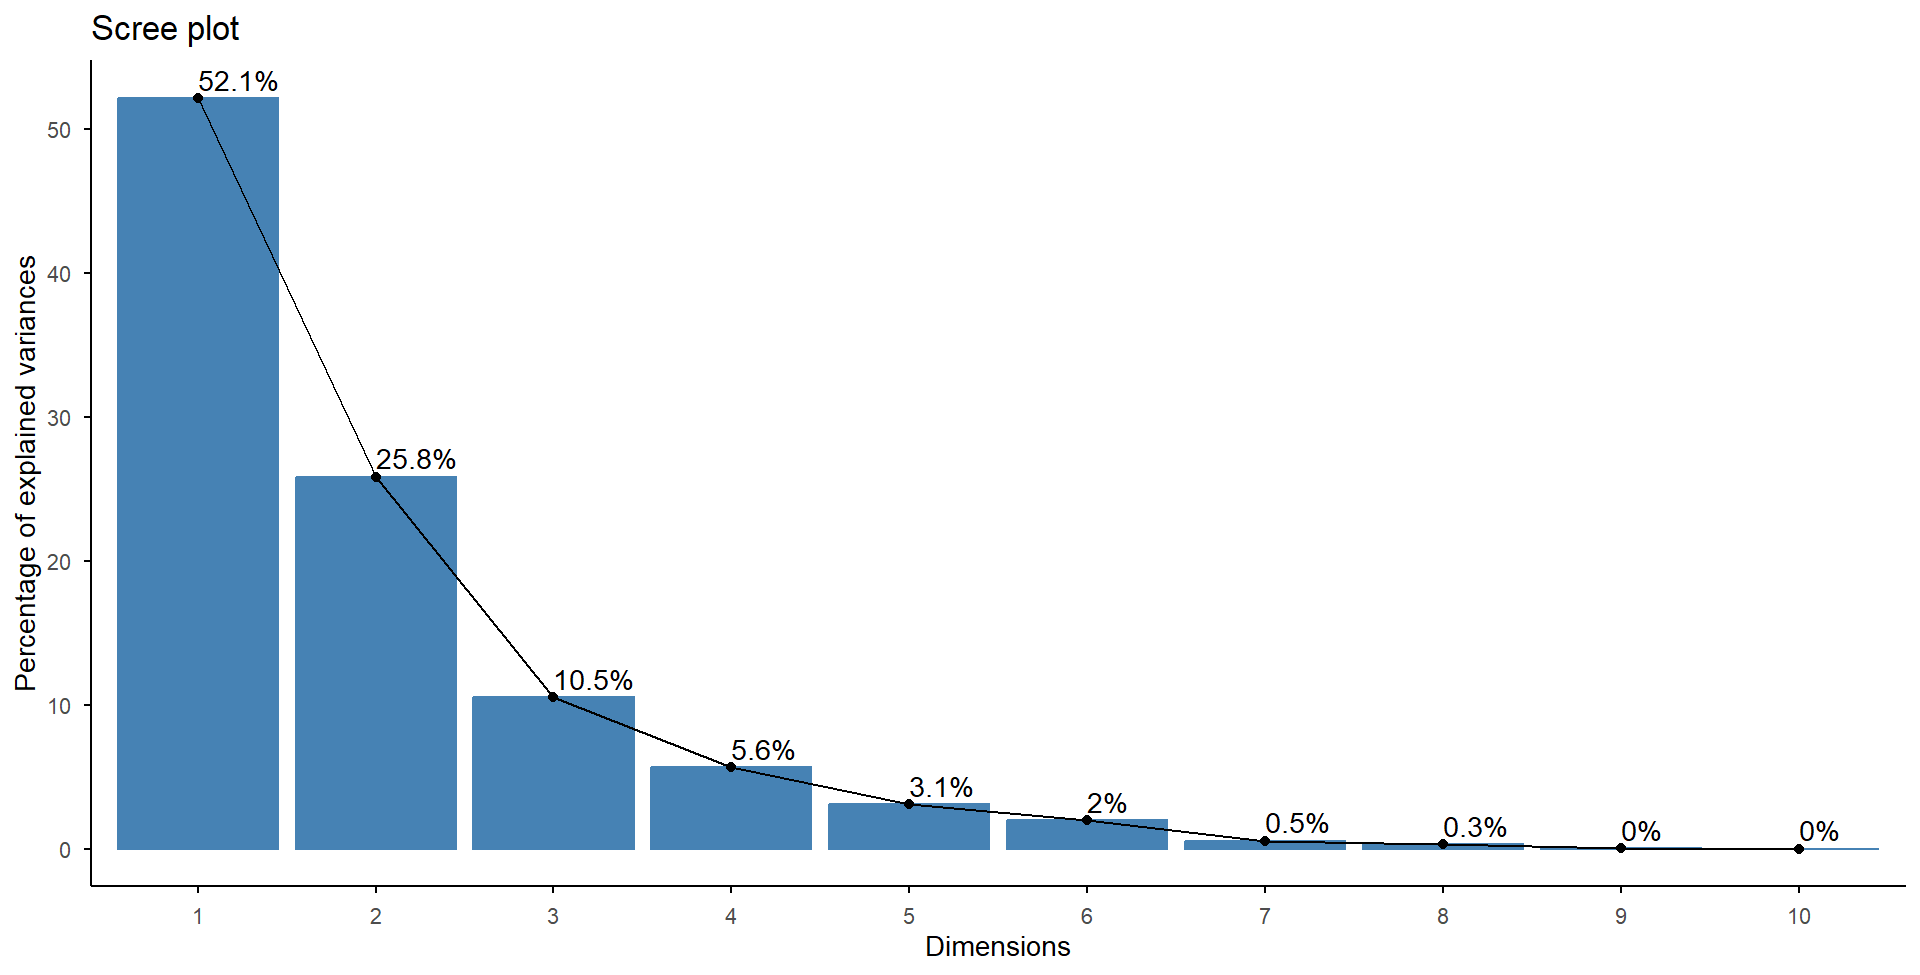
\includegraphics[width=0.8\textwidth]{figuras/Sedimentación.png}
        \caption{\label{figScree}Gráfico de sedimentación.}
        \end{figure}
        
        La Figura~\ref{figContriDim1} muestra la contribución relativa de cada variable original a la primera componente principal (PC1). Se observa que las variables \textit{Frequency}, \textit{Utilidad bruta}, \textit{Valor bruto}, \textit{SKUs distintos}, \textit{Monetary} y \textit{Valor neto} presentan contribuciones individuales superiores al umbral del 10\%, lo que indica que estas variables son las principales responsables de la variabilidad capturada por esta dimensión.

        El patrón de contribuciones observado en la Figura~\ref{figContriDim1} permite interpretar PC1 como un eje asociado al \emph{comportamiento económico agregado del cliente}. Esta componente sintetiza de manera conjunta la recurrencia de compra (\textit{Frequency}), la magnitud del gasto (\textit{Monetary}), el volumen económico generado (\textit{Valor bruto} y \textit{Valor neto}), la rentabilidad (\textit{Utilidad bruta}) y la amplitud del portafolio adquirido (\textit{SKUs distintos}). En consecuencia, valores elevados de PC1 corresponden a clientes con relaciones comerciales intensivas y de alto valor económico, mientras que valores bajos reflejan perfiles con baja intensidad transaccional.

        La Figura~\ref{figContriDim2} presenta las contribuciones de las variables a la segunda componente principal (PC2). En este caso, las variables con contribuciones superiores al 10\% son \textit{Costo total}, \textit{Descuentos}, \textit{Monetary}, \textit{Cantidad} y \textit{Valor neto}.

        A diferencia de PC1, la segunda componente captura una dimensión asociada a la \emph{estructura del gasto y su relación con costos y descuentos}. En particular, PC2 discrimina entre clientes que, aun presentando niveles similares de gasto monetario, difieren en la cantidad adquirida, en los costos asociados a sus compras y en la intensidad del uso de descuentos. Puntuaciones elevadas en esta dimensión reflejan perfiles con mayor volumen físico, mayores costos y una mayor incidencia de descuentos, mientras que puntuaciones bajas corresponden a estructuras de compra más simples o menos dependientes de incentivos comerciales.
        
        \begin{figure}[H]
        \centering
        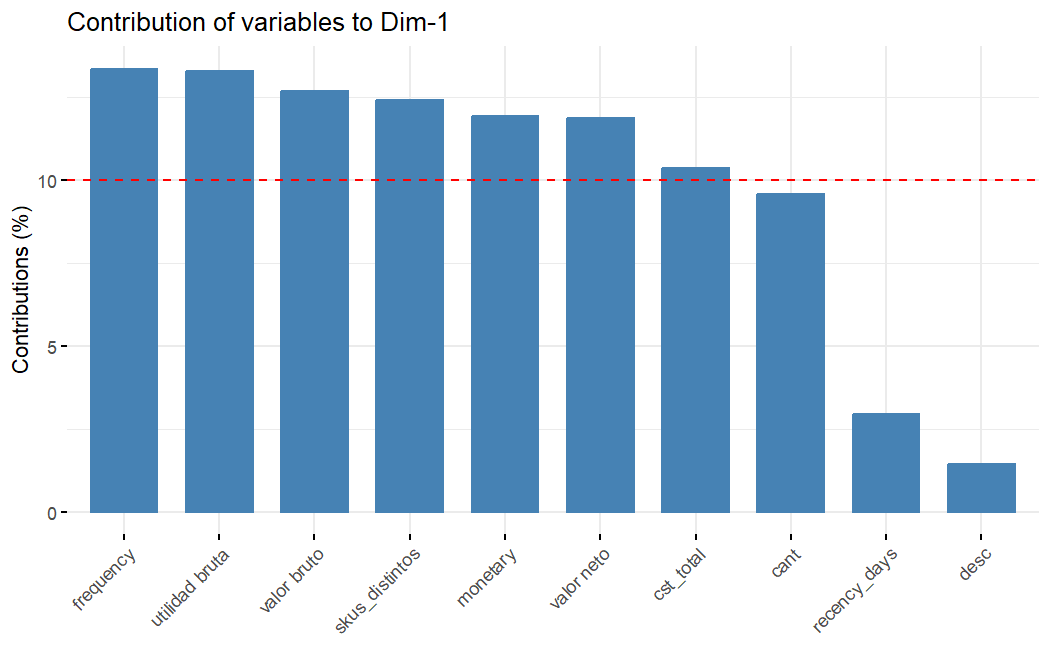
\includegraphics[width=0.8\textwidth]{figuras/Contri_Dim1.png}
        \caption{\label{figContriDim1}Contribución de las variables a la componente PC1.}
        \end{figure}
        
        \begin{figure}[H]
        \centering
        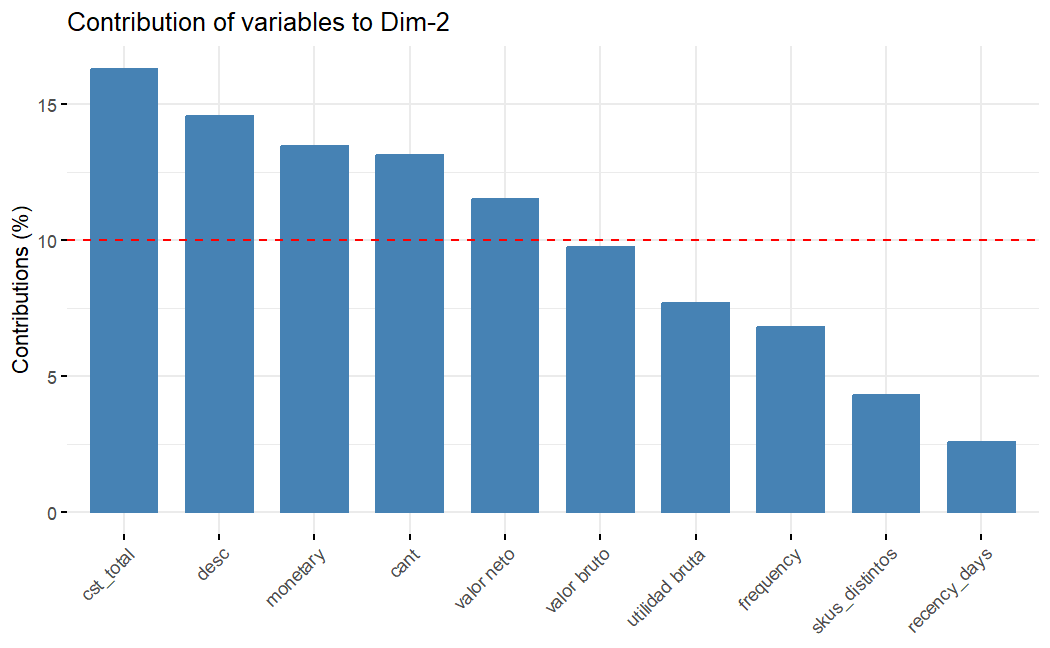
\includegraphics[width=0.8\textwidth]{figuras/Contri_Dim2.png}
        \caption{\label{figContriDim2}Contribución de las variables a la componente PC2.}
        \end{figure}
        
        La interpretación conjunta de ambas componentes se refuerza mediante el análisis del círculo de correlación presentado en la Figura~\ref{figPCAvars}, donde se visualizan simultáneamente la dirección y la magnitud de las cargas de cada variable en el plano definido por PC1 y PC2.
        
        \begin{figure}[H]
        \centering
        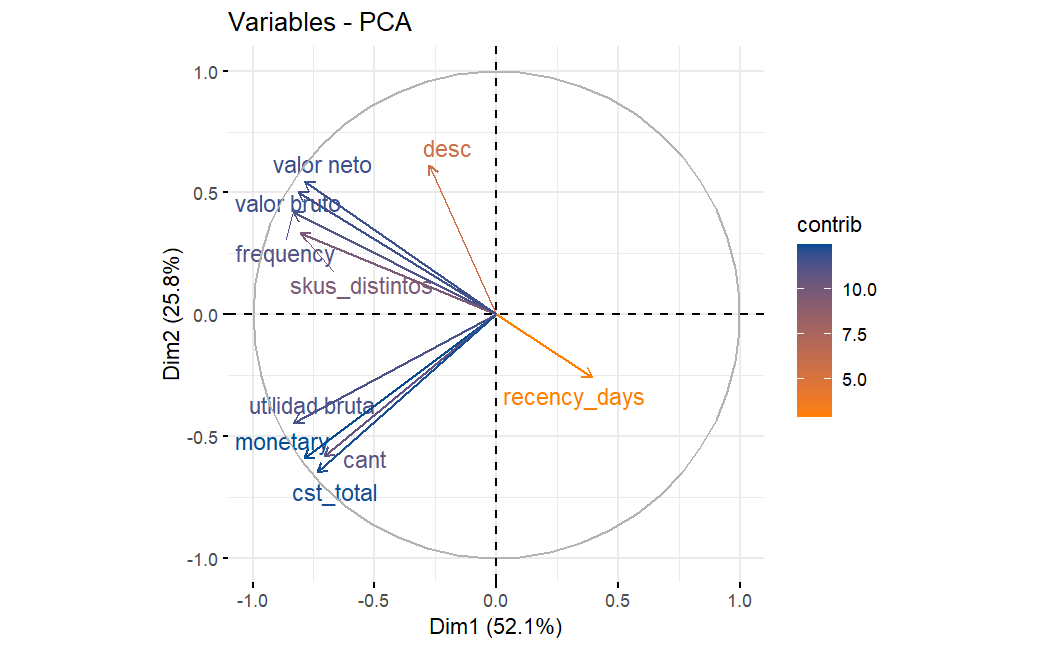
\includegraphics[width=0.8\textwidth]{figuras/Variables PCA.png}
        \caption{\label{figPCAvars}Círculo de correlación de las variables en el plano PC1--PC2.}
        \end{figure}
        
        En la Figura~\ref{figPCAvars} se observa que las variables \textit{Costo total}, \textit{Monetary}, \textit{Cantidad} y \textit{Utilidad bruta} apuntan en direcciones muy similares, lo que confirma una alta correlación estructural entre ellas y respalda empíricamente los resultados del análisis de correlación bivariada. Esta superposición justifica la conservación de una única variable representativa de esta dimensión económica, en particular \textit{Monetary}, dada su interpretación directa y su rol central dentro del esquema RFM.
        
        De manera análoga, las variables \textit{Valor bruto}, \textit{Valor neto} y \textit{Frequency} presentan una alineación estrecha, lo que indica que capturan información parcialmente redundante asociada al tamaño y recurrencia de la relación comercial. En este contexto, la retención de \textit{Frequency} permite preservar una medida directa de recurrencia conductual, mientras que \textit{Valor neto} aporta información complementaria sobre el monto efectivamente pagado tras la aplicación de descuentos.
        
        Finalmente, las variables \textit{Descuentos} y \textit{Recency} aparecen relativamente aisladas en el espacio factorial, con ángulos amplios respecto al resto de variables. Este patrón indica que aportan información adicional no redundante, asociada respectivamente a la política comercial aplicada al cliente y al tiempo transcurrido desde la última compra. En consecuencia, su inclusión resulta relevante para capturar dimensiones del comportamiento del cliente que no están explicadas exclusivamente por el volumen económico.
        
        Los resultados del PCA confirman la existencia de una estructura latente de baja dimensionalidad dominada por dos ejes principales: (i) una dimensión asociada a la intensidad y valor económico global del cliente (PC1) y (ii) una dimensión vinculada a la estructura del gasto, los costos y la sensibilidad a descuentos (PC2). Estas conclusiones son coherentes con los resultados del análisis de asociación previo y respaldan empíricamente las decisiones de selección y depuración de variables adoptadas antes del modelamiento del \emph{pogit}.

\subsection{Análisis de conglomerados mediante K-means}
        Con el objetivo de identificar segmentos homogéneos de clientes a partir de su comportamiento transaccional, se aplicó el algoritmo de agrupación
        \emph{K-means} sobre el conjunto de entrenamiento, utilizando exclusivamente las variables cuantitativas previamente seleccionadas: \textit{Monetary},
        \textit{Frequency}, \textit{Recency}, \textit{Descuentos} y \textit{Cantidad}.
        Todas las variables fueron transformadas y estandarizadas según lo descrito en la sección metodológica, garantizando comparabilidad en escala y evitando la dominancia de variables con mayor magnitud.
        
        La selección del número óptimo de clústeres \(k\) se realizó mediante el uso complementario del Método del Codo y del índice de Silhouette, con el fin de balancear compactación interna, separación entre grupos y parsimonia del modelo de segmentación.
        
        La Figura~\ref{figElbow} muestra la evolución de la suma de errores cuadráticos intra--clúster (WSS) en función de \(k\). Se observa una reducción pronunciada del WSS al pasar de \(k = 1\) a \(k = 3\), seguida de una disminución progresivamente más suave a partir de ese punto. Este cambio claro de pendiente identifica un “codo” alrededor de \(k = 3\), lo que sugiere que incrementos adicionales en el número de clústeres generan mejoras marginales en la compactación interna.
        
        De forma complementaria, la Figura~\ref{figSilhouette} presenta el valor promedio del índice de Silhouette para distintos valores de \(k\). El índice alcanza sus valores máximos para \(k = 2\), \(k = 3\) y \(k = 4\), con valores comprendidos entre 0.460 y 0.470, lo que indica una cohesión interna adecuada y una separación razonable entre grupos. A partir de \(k = 5\), el índice desciende de manera marcada hasta valores cercanos a 0.320, evidenciando una pérdida sustancial de calidad en la partición.

         Considerando conjuntamente ambos criterios, se seleccionó \(k = 4\) como una solución de compromiso entre parsimonia, calidad del agrupamiento y capacidad interpretativa de los segmentos resultantes. Esta elección permite capturar heterogeneidad relevante en el comportamiento de los clientes sin incurrir en sobresegmentación.

        \begin{figure}[H]
        \centering
        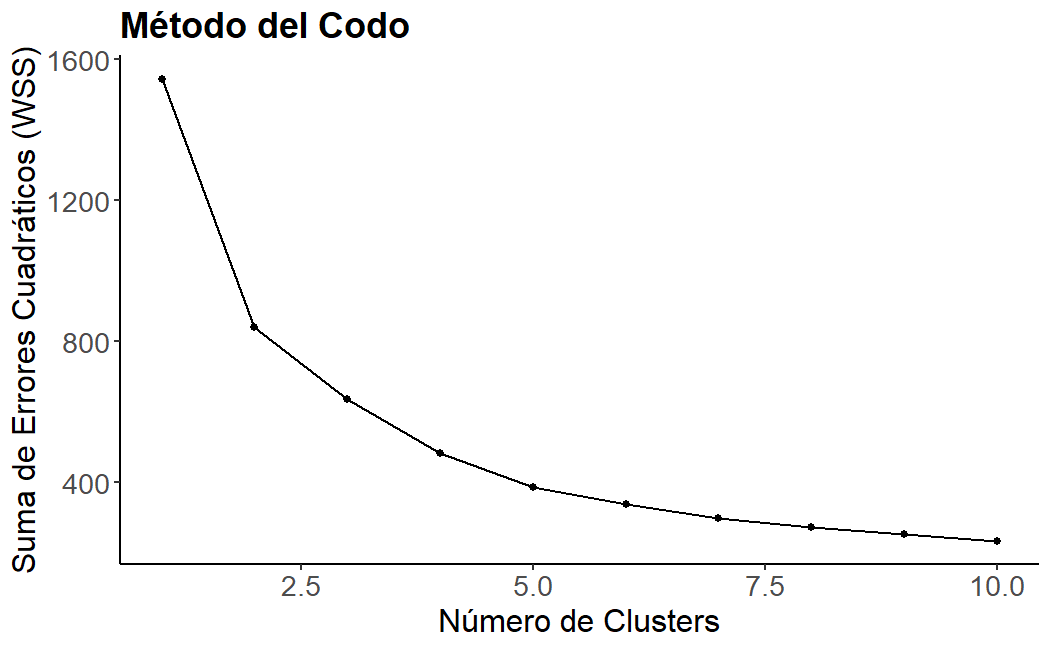
\includegraphics[width=0.8\textwidth]{figuras/Método del Codo.png}
        \caption{\label{figElbow}Método del Codo para la selección del número de clústeres.}
        \end{figure}
        
        \begin{figure}[H]
        \centering
        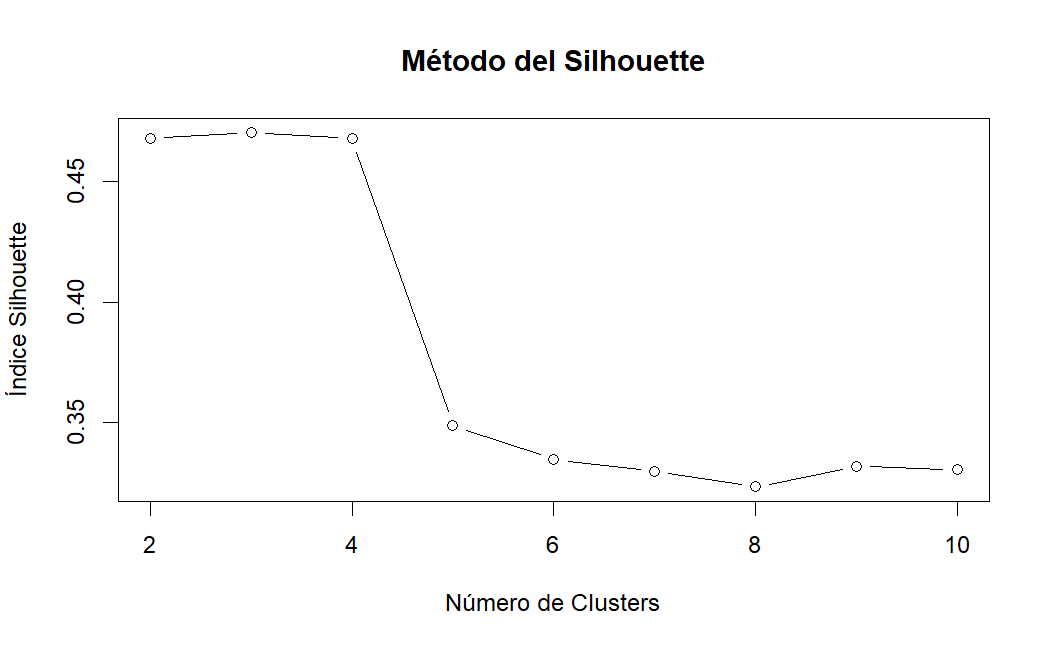
\includegraphics[width=0.8\textwidth]{figuras/Método de Silhoutte.png}
        \caption{\label{figSilhouette}Índice de Silhouette en función del número de clústeres.}
        \end{figure}
        
       
        La Tabla~\ref{figclust} presenta las medianas estandarizadas de las variables utilizadas para cada uno de los cuatro clústeres identificados. Dado que los valores corresponden a \emph{z-scores}, pueden interpretarse como desviaciones respecto a la media global del conjunto de entrenamiento.

         Por ejemplo, el valor 2.157 en la variable \textit{Monetary} para el Clúster 4 indica un nivel de gasto superior en más de dos desviaciones estándar respecto a la media, mientras que el valor -1.179 observado en el Clúster 3 refleja un gasto sustancialmente inferior al promedio.
        
        La Figura~\ref{figClusterPlot} muestra la proyección de los clústeres en el plano definido por las dos primeras componentes principales, las cuales explican conjuntamente aproximadamente el 78\% de la varianza total. La separación visual observada respalda la coherencia de la partición y la capacidad discriminante del conjunto de variables utilizadas.
        
        \begin{table}[H]
        \centering
        \caption{Medianas estandarizadas por clúster (K-means).}
        \label{figclust}
        \begin{tabular}{c c c c c c}
        \hline
        \textbf{Clúster} & \textbf{Monetary} & \textbf{Frequency} &
        \textbf{Recency} & \textbf{Descuentos} & \textbf{Cantidad} \\
        \hline
        1 & 0.855 & 1.470 & -1.349 & 0.857 & 0.676 \\
        2 & -0.430 & -0.727 & 0.541 & 0.261 & -0.515 \\
        3 & -1.179 & -0.727 & 0.673 & -2.225 & -0.090 \\
        4 & 2.157 & 1.219 & -0.417 & -2.225 & 2.301 \\
        \hline
        \end{tabular}
        \end{table}
        
       
        
        \begin{figure}[H]
        \centering
        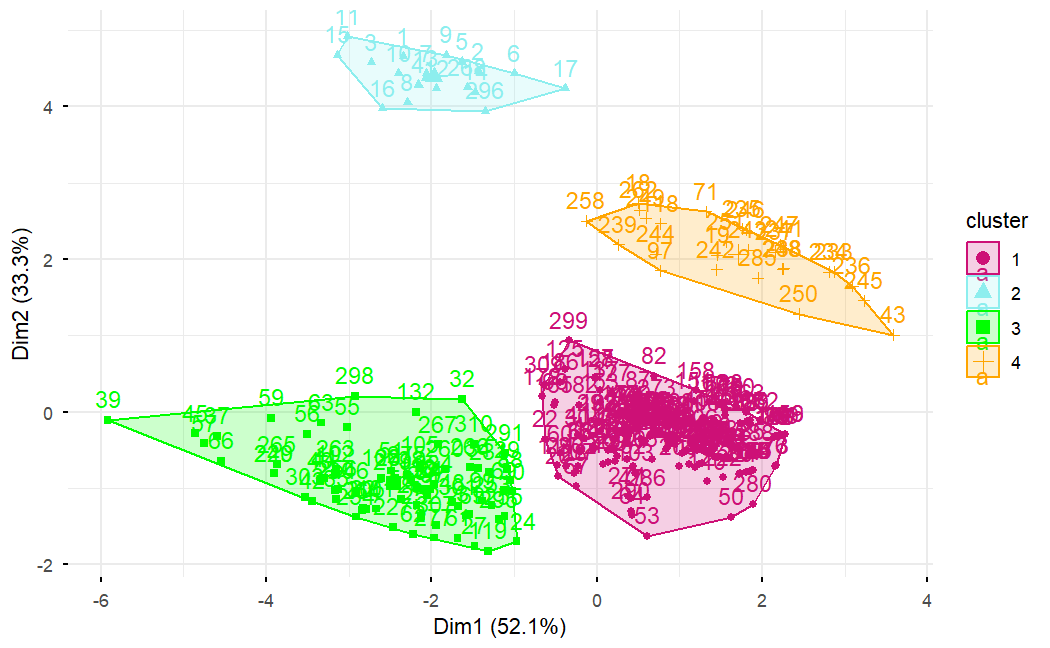
\includegraphics[width=0.8\textwidth]{figuras/Cluster Plot.png}
        \caption{\label{figClusterPlot}Proyección de los clústeres en el espacio de las dos primeras componentes principales.}
        \end{figure}
        
        A partir de los valores resumidos en la Tabla~\ref{figclust} y de la evidencia gráfica, se identifican perfiles claramente diferenciados. El Clúster 1 agrupa clientes con gasto y frecuencia superiores a la media y baja recencia, lo que indica relaciones comerciales activas y estables. El Clúster 2 concentra clientes de bajo valor, con baja frecuencia y mayor tiempo desde la última compra, representando un segmento con riesgo de abandono. El Clúster 3 presenta los niveles más bajos de gasto y frecuencia, junto con alta recencia, reflejando una relación comercial debilitada. Finalmente, el Clúster 4 se distingue por valores
        extremadamente altos de gasto, frecuencia y cantidad, baja recencia y mínima incidencia de descuentos, concentrando una proporción sustancial del valor total a pesar de su tamaño reducido, en línea con el principio de Pareto.
        
        Estos resultados confirman que el algoritmo K-means, aplicado de manera adecuada sobre variables cuantitativas y restringido al conjunto de entrenamiento, permite identificar segmentos estadísticamente diferenciados y económicamente interpretables, los cuales serán utilizados posteriormente como insumo descriptivo y como apoyo para la especificación del modelo de \emph{SoW}.

\subsection{Segmentación mediante K-medoids con distancia de Gower (variables mixtas)}
        Con el objetivo de identificar segmentos homogéneos de clientes considerando simultáneamente información transaccional y atributos categóricos, se aplicó el algoritmo de agrupación \emph{K-medoids} utilizando la distancia de Gower. Este procedimiento se implementó exclusivamente sobre el conjunto de entrenamiento, de acuerdo con el diseño experimental descrito en la sección metodológica. La
        distancia de Gower permite integrar variables continuas y cualitativas dentro de una única matriz de disimilitud, lo que resulta adecuado para la segmentación de clientes en presencia de datos mixtos.
        
        \begin{figure}[H]
        \centering
        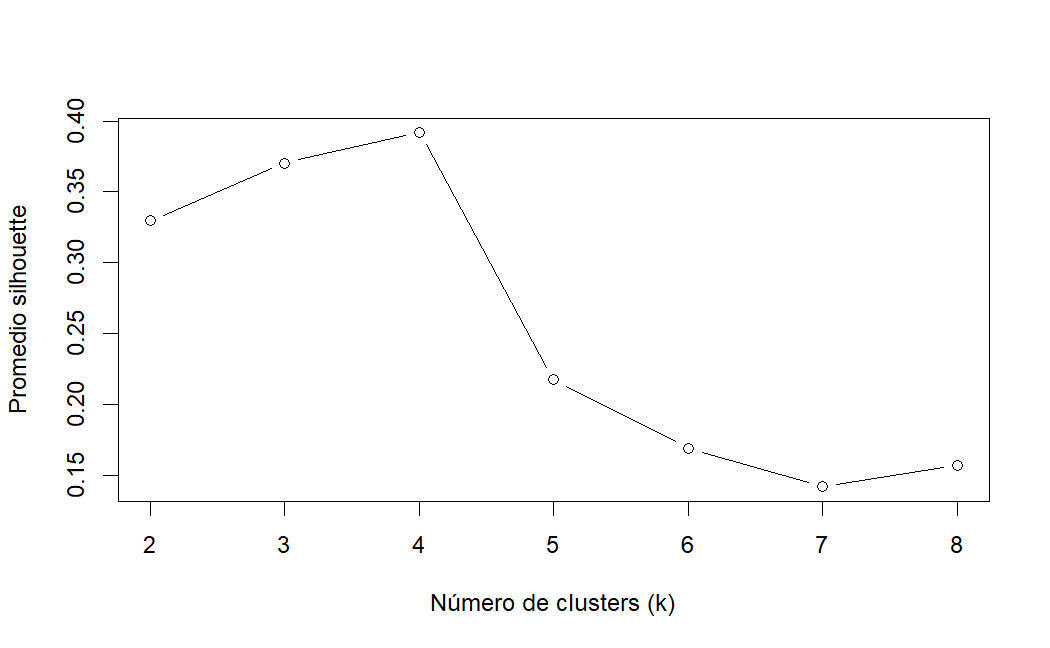
\includegraphics[width=0.8\textwidth]{figuras/Siluet.png}
        \caption{\label{figSilhouetteGower}Índice Silhouette promedio para K-medoids con distancia de Gower.}
        \end{figure}
        
        La Figura~\ref{figSilhouetteGower} presenta la evolución del índice Silhouette promedio para distintos valores del número de clústeres \(k\). Se observa que el valor máximo se alcanza en \(k = 4\), con un índice comprendido aproximadamente entre 0.39 y 0.40. A partir de este punto, el índice disminuye de forma sostenida, lo que indica una pérdida progresiva de cohesión interna y separación entre grupos al incrementar el número de clústeres. En consecuencia, la solución con cuatro clústeres se identifica como aquella que ofrece el mejor compromiso entre calidad del agrupamiento y parsimonia del modelo.
        
        Si bien estos valores son inferiores a los umbrales comúnmente asociados con estructuras de clústeres altamente definidas (superiores a 0.50), resultan consistentes con la complejidad inherente a la segmentación basada en variables mixtas. En particular, la inclusión de atributos categóricos suele reducir la separabilidad geométrica entre observaciones, lo que se refleja en valores moderados del índice Silhouette incluso cuando existe estructura latente en los
        datos.
        
        \begin{figure}[H]
        \centering
        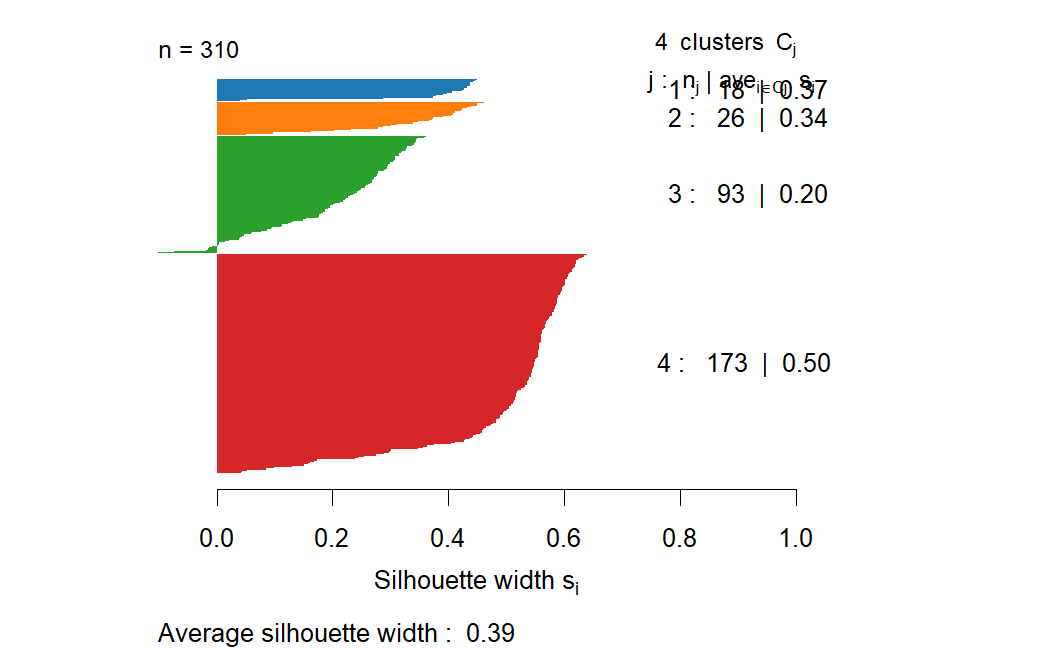
\includegraphics[width=0.8\textwidth]{figuras/KMEDOIDS.png}
        \caption{\label{figSilhouette4}Silhouette plot para la solución con \(k = 4\).}
        \end{figure}
        
        La Figura~\ref{figSilhouette4} muestra el \emph{Silhouette plot} correspondiente a la partición con cuatro clústeres. El índice Silhouette promedio global es 0.39, lo que indica una estructura de agrupamiento moderadamente consistente, aunque con heterogeneidad relevante entre los clústeres individuales.
        
        En particular, el clúster 4 presenta el mayor valor promedio de Silhouette, cercano a 0.50, lo que evidencia una elevada cohesión interna y una separación clara respecto a los demás grupos. Los clústeres 1 y 2 exhiben valores promedio de 0.37 y 0.34, respectivamente, lo que sugiere una calidad aceptable, aunque con fronteras menos definidas. En contraste, el clúster 3 presenta un valor promedio cercano a 0.20, indicando una estructura débil y un alto grado de solapamiento con
        otros clústeres, lo que sugiere una menor homogeneidad interna y una asignación menos estable de las observaciones.

        La Figura~\ref{figPAMGower} refuerza visualmente los resultados cuantitativos derivados del índice Silhouette. El clúster 4 se observa claramente compacto y bien separado, en coherencia con su alto valor promedio de Silhouette. Por el contrario, el clúster 3 presenta una dispersión considerable, consistente con su
        bajo índice de Silhouette, lo que evidencia una separación poco definida respecto a los demás grupos.
        
        Los clústeres 1 y 2, aunque de menor tamaño relativo, muestran una separación visual razonable y una dispersión moderada, lo que sugiere la existencia de segmentos de nicho caracterizados por combinaciones particulares de atributos categóricos y patrones transaccionales diferenciados.
        
        \begin{figure}[H]
        \centering
        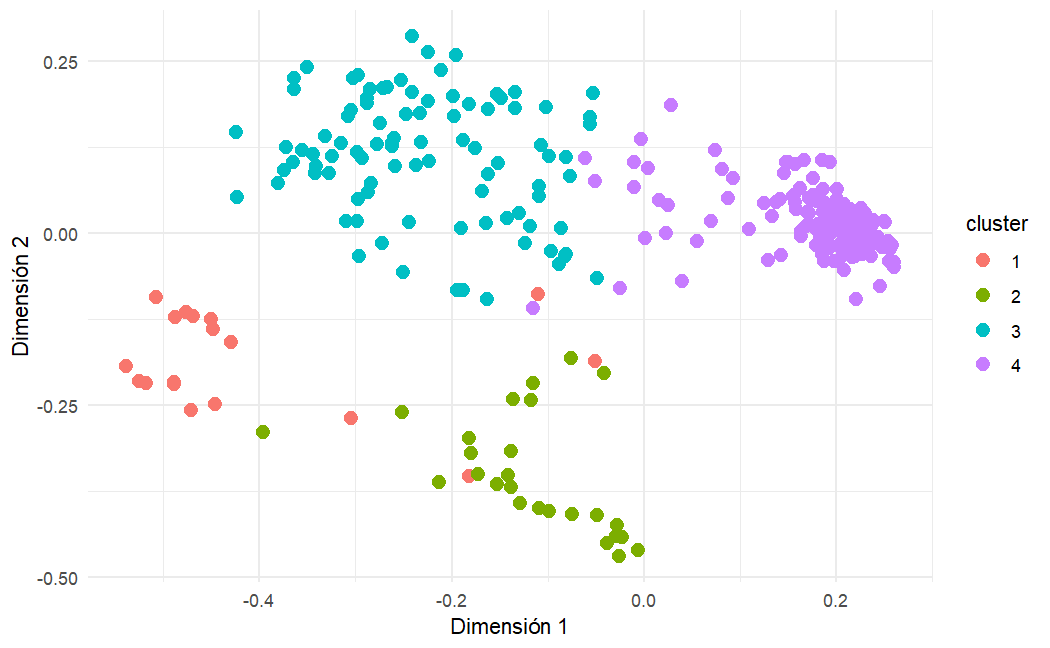
\includegraphics[width=0.8\textwidth]{figuras/CLUSTER.png}
        \caption{\label{figPAMGower}Representación bidimensional del agrupamiento PAM con distancia de Gower.}
        \end{figure}
        
        Los resultados obtenidos mediante K-medoids con distancia de Gower indican que la solución con cuatro clústeres captura una estructura relevante en los datos mixtos del conjunto de entrenamiento, permitiendo identificar segmentos con distintos niveles de cohesión y separabilidad. 

        Con el fin de evaluar la estabilidad y utilidad práctica de las segmentaciones obtenidas, los modelos de agrupamiento mediante K-means y K-medoids se aplican sobre el conjunto de prueba, asignando cada cliente a uno de los segmentos definidos a partir del conjunto de entrenamiento. Estas agrupaciones permitirán analizar la coherencia de los perfiles de clientes fuera de la muestra utilizada para la estimación, así como contrastar la segmentación basada en variables transaccionales y mixtas con la segmentación emergente del comportamiento observado. En particular, los clústeres asignados en el conjunto de prueba se compararán con la clasificación visual derivada del
        gráfico tipo \emph{bubble} de \emph{SoW} frente a
        \emph{SioW}, ambos predichos por el modelo pogit, lo que permitirá evaluar en qué medida los segmentos identificados por métodos no supervisados se alinean con patrones económicos
        predichos de participación y potencial de cartera. 

%--------------------------------------------------
\section{Resultados de la estimación del modelo \emph{pogit}}
    Esta sección presenta los resultados empíricos de la estimación del modelo \emph{pogit} aplicado al comportamiento de compra de los clientes empresariales de la Empresa Distribuidora de Biblias y Literatura Cristiana. El análisis se centra en la evidencia estadística asociada a los coeficientes estimados para los componentes de participación en la billetera (SoW) y tamaño de la billetera (SioW), así como en la consistencia de dichos resultados a través de distintas especificaciones del modelo.

    Dado el carácter latente de las variables SoW y SioW y la ausencia de valores empíricos observables de referencia, los resultados se evalúan desde una perspectiva inferencial y estructural. En particular, el énfasis se coloca en la significancia estadística, la estabilidad de los coeficientes y su coherencia con los mecanismos teóricos subyacentes al modelo \emph{pogit}, más que en criterios de validación predictiva tradicionales.

\subsection{Resultados con variables transaccionales originales}
    Las Tablas~\ref{tab:pogit_coefficients_full_version1}–\ref{tab:pogit_coefficients_version6} reportan los resultados obtenidos a partir de especificaciones del modelo \emph{pogit} construidas con variables transaccionales originales, previamente sometidas a procesos de limpieza y estandarización. En todas estas especificaciones, el componente de asignación (SoW) se modela mediante variables del tipo RFM, mientras que el componente de intensidad (SioW) incorpora distintos subconjuntos de covariables categóricas orientadas a capturar heterogeneidad estructural entre clientes.

    En el componente de participación en la billetera, la variable \textit{Monetary} exhibe coeficientes positivos en todas las especificaciones reportadas y alcanza significancia estadística en las versiones reducidas del modelo (Tablas~\ref{tab:pogit_coefficients_reduced_version3}, \ref{tab:pogit_coefficients_reduced_version4} y \ref{tab:pogit_coefficients_version5}). Este patrón indica que un mayor gasto histórico del cliente en la empresa focal se asocia sistemáticamente con una mayor fracción de su gasto total en la categoría asignada a dicha empresa, en línea con la interpretación económica de la SoW como una medida de preferencia relativa.

    Por el contrario, las variables \textit{Frequency} y \textit{Recency} no presentan efectos estadísticamente significativos en la mayoría de las especificaciones consideradas (Tablas~\ref{tab:pogit_coefficients_reduced_version3}–\ref{tab:pogit_coefficients_version6}). Este resultado sugiere que, una vez controlado el nivel agregado de gasto histórico, la frecuencia de compra y la antigüedad de la última transacción aportan información limitada para explicar la asignación relativa del gasto hacia la empresa focal.

    En el componente de intensidad (SioW), ninguna de las especificaciones basadas en variables originales presenta coeficientes individuales estadísticamente significativos, y los interceptos estimados tampoco resultan significativos en la mayoría de los casos. 

    La comparación entre la especificación completa (Tabla~\ref{tab:pogit_coefficients_full_version1}) y las versiones reducidas del modelo indica que una parametrización más parsimoniosa del componente de intensidad es suficiente para obtener estimaciones estables del componente de asignación, sin alterar de manera sustantiva los coeficientes asociados a las variables RFM en la SoW.

\subsection{Resultados con reducción de dimensionalidad mediante PCA}
    Las Tablas~\ref{tab:pogit_coefficients_version7}–\ref{tab:pogit_coefficients_version9} presentan los resultados correspondientes a especificaciones en las que el componente de asignación (SoW) se modela a partir de componentes principales obtenidas mediante Análisis de Componentes Principales (PCA).

    En las especificaciones reportadas en las Tablas~\ref{tab:pogit_coefficients_version7} y \ref{tab:pogit_coefficients_version8}, la primera componente principal (PC1) exhibe un coeficiente negativo y estadísticamente significativo en el componente SoW, mientras que la segunda componente (PC2) presenta un coeficiente positivo con significancia marginal. Este patrón sugiere que clientes con mayor intensidad económica global tienden a diversificar su gasto entre múltiples proveedores, reduciendo la fracción asignada a la empresa focal, mientras que ciertas estructuras del gasto asociadas a relaciones comerciales más específicas se vinculan con una mayor concentración del gasto en dicha empresa.

    En estas mismas especificaciones, el componente de intensidad (SioW) no presenta coeficientes individuales estadísticamente significativos, en concordancia con los resultados observados en las especificaciones basadas en variables originales.

    Un resultado cualitativamente distinto emerge en la especificación más parsimoniosa basada en PCA (Tabla~\ref{tab:pogit_coefficients_version9}). En este caso, los coeficientes asociados a las componentes principales PC1 y PC2 no resultan estadísticamente significativos en el componente de asignación (SoW). En contraste, la variable indicadora de tipo de empresa (nacional) presenta un coeficiente negativo y estadísticamente significativo en el componente de intensidad (SioW). Este resultado indica que, aun bajo una especificación mínima, persisten diferencias estructurales en el tamaño de la billetera asociadas al tipo de empresa del cliente.

    En este contexto, la pérdida de significancia de PC1 y PC2 en el componente SoW no debe interpretarse como evidencia de irrelevancia de las dimensiones latentes del comportamiento económico del cliente, sino como una limitación de dichas componentes para identificar el mecanismo de asignación cuando el componente de intensidad se encuentra altamente restringido.

\subsection{Selección de la especificación de referencia}
    Los resultados muestran que las especificaciones basadas en variables originales y aquellas que incorporan reducción de dimensionalidad mediante PCA conducen a inferencias coherentes sobre la participación en la billetera, particularmente en lo relativo al rol del gasto histórico y a la estabilidad del componente de asignación. No obstante, difieren en el grado de parsimonia y en la forma en que caracterizan el componente de intensidad.
    
    La especificación presentada en la Tabla~\ref{tab:pogit_coefficients_reduced_version3} se adopta como referencia para el análisis de estimaciones de SioW versus SoW, dado que ofrece una caracterización estable y estructural del tamaño de la billetera basada en atributos del cliente y de la categoría de producto, sin introducir dependencias estacionales ni concentrar artificialmente la heterogeneidad del componente SioW en una única variable. Esta elección proporciona una base inferencial clara y reproducible para el examen conjunto de las estimaciones de SoW y SioW en la siguiente etapa del análisis.

\begin{table}[ht]
    \centering
    \begin{threeparttable}
    \caption{Coeficientes estimados del modelo \emph{pogit} con especificación completa. Se reportan estimaciones puntuales y valores $p$ para las covariables cuantitativas del componente de participación de cartera (SoW). Las covariables categóricas incluidas en ambos componentes del modelo se estiman conjuntamente pero se omiten del reporte numérico por brevedad.}
    \label{tab:pogit_coefficients_full_version1}
    
    \begin{tabular}{
    l
    S[table-format=2.3]
    S[table-format=1.3]
    }
    \toprule
    Covariable &
    {Estimación} &
    {$p$-valor} \\
    \midrule
    
    \multicolumn{3}{l}{\textbf{SoW}}\\
    \addlinespace
    
    Intercepto
    & -5.496
    & 0.510 \\
    
    Monetary 
    & 5.676
    & 0.625 \\
    
    Frequency 
    & 0.766
    & 0.656 \\
    
    Recency 
    & -0.504
    & 0.729 \\
    
    Condiciones del cliente$^{a}$
    & {} & {} \\
    
    \addlinespace
    \midrule
    \addlinespace
    
    \multicolumn{3}{l}{\textbf{SioW}}\\
    \addlinespace
    
    Intercepto
    & -0.881
    & 0.934 \\
    
    Tipo de cliente$^{b}$
    & {} & {} \\
    
    Ubicación geográfica$^{c}$
    & {} & {} \\
    
    Categoría de producto$^{d}$
    & {} & {} \\
    
    Indicadores mensuales$^{e}$
    & {} & {} \\
    
    Tipo de empresa$^{f}$
    & {} & {} \\
    
    \bottomrule
    \end{tabular}
    
    \begin{tablenotes}[flushleft]
    \footnotesize
    \item $^{a}$ Indicadores de condición del cliente: consignación, crédito, distribuidor, donación, iglesia y librería.
    \item $^{b}$ Indicador de cliente nacional frente a internacional.
    \item $^{c}$ Variables indicadoras de departamento y ciudad (ubicaciones nacionales e internacionales).
    \item $^{d}$ Indicadores de categoría de producto: fina, línea y semifina.
    \item $^{e}$ Variables indicadoras del mes del año.
    \item $^{f}$ Indicadores de tipo de empresa: editorial, educativa, fundación y religiosa.
    \end{tablenotes}
    
    \end{threeparttable}
\end{table}


\begin{table}[ht]
    \centering
    \begin{threeparttable}
    \caption{Coeficientes estimados del modelo \emph{pogit} (Versión: SoW = Intercepto + RFM; SioW = Intercepto + Ubicación + Tipo de empresa). Se reportan las estimaciones puntuales y valores-$p$ para las covariables cuantitativas incluidas en el componente SoW. Las variables categóricas incluidas en el componente SioW se incorporan en la estimación pero se omiten del reporte numérico por brevedad.}
    \label{tab:pogit_coefficients_reduced_version2}
    
    \begin{tabular}{
    l
    S[table-format=2.3, table-number-alignment=right]
    S[table-format=1.3, table-number-alignment=right]
    }
    \toprule
    Covariable &
    {Estimación} &
    {$p$-valor} \\
    \midrule
    
    \multicolumn{3}{l}{\textbf{SoW}}\\
    \addlinespace
    
    Intercepto
    & -4.734
    & 0.005 \\
    
    Monetary
    & 5.503
    & 0.079 \\
    
    Frequency
    & 0.655
    & 0.398 \\
    
    Recency
    & -0.219
    & 0.856 \\
    
    \addlinespace
    \midrule
    \addlinespace
    
    \multicolumn{3}{l}{\textbf{SioW}}\\
    \addlinespace
    
    Intercepto
    & 0.372
    & 0.707 \\
    
    Ubicación geográfica$^{a}$
    & {} & {} \\
    
    Tipo de empresa$^{b}$
    & {} & {} \\
    
    \bottomrule
    \end{tabular}
    
\begin{tablenotes}[flushleft]
    \footnotesize
    \item $^{a}$ Variables indicadoras de ubicación geográfica a nivel de departamento y ciudad, tanto nacionales como internacionales.
    \item $^{b}$ Variables indicadoras del tipo de empresa: editorial, educativa, fundación y religiosa.
\end{tablenotes}
    
    \end{threeparttable}
\end{table}


\begin{table}[ht]
    \centering
    \begin{threeparttable}
    \caption{Coeficientes estimados del modelo \emph{pogit} (Versión: SoW = Intercepto + RFM; SioW = Intercepto + Categoría de producto + Tipo de cliente). Se reportan estimaciones puntuales y valores $p$ para las covariables cuantitativas del componente SoW. Las variables categóricas del componente de intensidad (SioW) se incluyen en la estimación pero se omiten de la presentación numérica por brevedad.}
    \label{tab:pogit_coefficients_reduced_version3}
    
    \begin{tabular}{
    l
    S[table-format=2.3]
    S[table-format=1.3]
    }
    \toprule
    Covariable &
    {Estimación} &
    {$p$-valor} \\
    \midrule
    
    \multicolumn{3}{l}{\textbf{SoW}}\\
    \addlinespace
    
    Intercepto
    & -5.144
    & 0.000 \\
    
    Monetary
    & 4.681
    & 0.003 \\
    
    Frequency
    & 0.687
    & 0.199 \\
    
    Recency
    & -0.053
    & 0.955 \\
    
    \addlinespace
    \midrule
    \addlinespace
    
    \multicolumn{3}{l}{\textbf{SioW}}\\
    \addlinespace
    
    Intercepto
    & 0.430
    & 0.414 \\
    
    Tipo de cliente / empresa$^{a}$
    & {} & {} \\
    
    Categoría de producto$^{b}$
    & {} & {} \\
    
    \bottomrule
    \end{tabular}
    
    \begin{tablenotes}[flushleft]
    \footnotesize
    \item $^{a}$ Indicadores del tipo de cliente y tipo de empresa: cliente nacional e indicadores de empresa (editorial, educativa, fundación, religiosa).
    \item $^{b}$ Indicadores de categoría de producto: fina, línea y semifina.
    \end{tablenotes}
    
    \end{threeparttable}
\end{table}

\begin{table}[ht]
    \centering
    \begin{threeparttable}
    \caption{Coeficientes estimados del modelo \emph{pogit} (Versión: SoW = Intercepto + RFM; SioW = Intercepto + Categoría de producto + Mes del año). Se reportan estimaciones puntuales y valores $p$ para las covariables cuantitativas del componente de participación de cartera (SoW). Las variables categóricas y estacionales del componente de intensidad (SioW) se incluyen en la estimación pero se omiten del reporte numérico por brevedad.}
    \label{tab:pogit_coefficients_reduced_version4}
    
    \begin{tabular}{
    l
    S[table-format=2.3]
    S[table-format=1.3]
    }
    \toprule
    Covariable &
    {Estimación} &
    {$p$-valor} \\
    \midrule
    
    \multicolumn{3}{l}{\textbf{SoW}}\\
    \addlinespace
    
    Intercepto
    & -4.834
    & 0.000 \\
    
    Monetary
    & 5.262
    & 0.001 \\
    
    Frequency
    & 0.598
    & 0.172 \\
    
    Recency
    & 0.130
    & 0.873 \\
    
    \addlinespace
    \midrule
    \addlinespace
    
    \multicolumn{3}{l}{\textbf{SioW}}\\
    \addlinespace
    
    Intercepto
    & 0.804
    & 0.084 \\
    
    Categoría de producto$^{a}$
    & {} & {} \\
    
    Mes del año$^{b}$
    & {} & {} \\
    
    \bottomrule
    \end{tabular}
    
    \begin{tablenotes}[flushleft]
    \footnotesize
    \item $^{a}$ Indicadores de categoría de producto: fina, línea y semifina.
    \item $^{b}$ Indicadores mensuales: enero a diciembre (estacionalidad anual).
    \end{tablenotes}
    
    \end{threeparttable}
\end{table}

\begin{table}[ht]
    \centering
    \begin{threeparttable}
    \caption{Coeficientes estimados del modelo \emph{pogit} (Versión: SoW = Intercepto + RFM; SioW = Intercepto + Categoría de producto). Se reportan estimaciones puntuales y valores $p$ para las covariables cuantitativas del componente de participación de cartera (SoW). Las covariables categóricas incluidas en ambos componentes del modelo se estiman conjuntamente pero se omiten del reporte numérico por brevedad.}
    \label{tab:pogit_coefficients_version5}
    
    \begin{tabular}{
    l
    S[table-format=2.3]
    S[table-format=1.3]
    }
    \toprule
    Covariable &
    {Estimación} &
    {$p$-valor} \\
    \midrule
    
    \multicolumn{3}{l}{\textbf{SoW}}\\
    \addlinespace
    
    Intercepto
    & -4.126
    & 0.004 \\
    
    Monetary
    & 6.305
    & 0.010 \\
    
    Frequency
    & 0.440
    & 0.466 \\
    
    Recency
    & -0.019
    & 0.984 \\
    
    \addlinespace
    \midrule
    \addlinespace
    
    \multicolumn{3}{l}{\textbf{SioW}}\\
    \addlinespace
    
    Intercepto
    & -0.603
    & 0.550 \\
    
    Categoría de producto$^{a}$
    & {} & {} \\
    
    \bottomrule
    \end{tabular}
    
    \begin{tablenotes}[flushleft]
    \footnotesize
    \item $^{a}$ Indicadores de categoría de producto: fina, línea y semifina.
    \end{tablenotes}
    
    \end{threeparttable}
\end{table}


\begin{table}[ht]
    \centering
    \begin{threeparttable}
    \caption{Coeficientes estimados del modelo \emph{pogit} (Versión: SoW = Intercepto + RFM; SioW = Intercepto + indicadores mensuales). Se reportan estimaciones puntuales y valores $p$ para las covariables cuantitativas del componente de participación de cartera (SoW). Las covariables categóricas del componente de intensidad (SioW) se estiman conjuntamente pero se omiten del reporte numérico por brevedad.}
    \label{tab:pogit_coefficients_version6}
    
    \begin{tabular}{
    l
    S[table-format=2.3]
    S[table-format=1.3]
    }
    \toprule
    Covariable &
    {Estimación} &
    {$p$-valor} \\
    \midrule
    
    \multicolumn{3}{l}{\textbf{SoW}}\\
    \addlinespace
    
    Intercepto
    & -4.834
    & 0.000 \\
    
    Monetary
    & 5.262
    & 0.001 \\
    
    Frequency
    & 0.598
    & 0.172 \\
    
    Recency
    & 0.130
    & 0.873 \\
    
    \addlinespace
    \midrule
    \addlinespace
    
    \multicolumn{3}{l}{\textbf{SioW}}\\
    \addlinespace
    
    Intercepto
    & 0.804
    & 0.084 \\
    
    Indicadores mensuales$^{a}$
    & {} & {} \\
    
    \bottomrule
    \end{tabular}
    
    \begin{tablenotes}[flushleft]
    \footnotesize
    \item $^{a}$ Variables indicadoras del mes del año.
    \end{tablenotes}
    
    \end{threeparttable}
\end{table}


\begin{table}[ht]
    \centering
    \begin{threeparttable}
    \caption{Coeficientes estimados del modelo \emph{pogit} (Versión: SoW = Intercepto + PC1 + PC2 + condiciones del cliente; SioW = Intercepto + Ubicación geográfica + Tipo de empresa). Se reportan las estimaciones puntuales y valores-$p$ para las covariables cuantitativas incluidas en el componente SoW. Las variables categóricas del componente SioW se incorporan en la estimación pero se omiten del reporte numérico por brevedad.}
    \label{tab:pogit_coefficients_version7}
    
    \begin{tabular}{
    l
    S[table-format=2.3, table-number-alignment=right]
    S[table-format=1.3, table-number-alignment=right]
    }
    \toprule
    Covariable &
    {Estimación} &
    {$p$-valor} \\
    \midrule
    
    \multicolumn{3}{l}{\textbf{SoW}}\\
    \addlinespace
    
    Intercepto
    & -5.167
    & 0.000 \\
    
    PC1
    & -2.997
    & 0.005 \\
    
    PC2
    & 2.066
    & 0.053 \\
    
    Condición: consignación
    & -0.468
    & 0.987 \\
    
    Condición: crédito
    & 1.793
    & 0.271 \\
    
    Condición: distribuidor
    & -8.612
    & 0.960 \\
    
    \addlinespace
    \midrule
    \addlinespace
    
    \multicolumn{3}{l}{\textbf{SioW}}\\
    \addlinespace
    
    Intercepto
    & 0.367
    & 0.068 \\
    
    Ubicación geográfica$^{a}$
    & {} & {} \\
    
    Tipo de empresa$^{b}$
    & {} & {} \\
    
    \bottomrule
    \end{tabular}
    
    \begin{tablenotes}[flushleft]
    \footnotesize
    \item $^{a}$ Variables indicadoras de ubicación geográfica agregada.
    \item $^{b}$ Indicadores de tipo de empresa.
    \end{tablenotes}
    
    \end{threeparttable}
\end{table}


\begin{table}[ht]
    \centering
    \begin{threeparttable}
    \caption{Coeficientes estimados del modelo \emph{pogit} (Versión: SoW = Intercepto + PC1 + PC2 + condiciones del cliente; SioW = Intercepto + Ubicación geográfica + Tipo de empresa + Categoría de producto). Se reportan las estimaciones puntuales y valores-$p$ para las covariables cuantitativas incluidas en el componente SoW. Las variables categóricas del componente SioW se incorporan en la estimación pero se omiten del reporte numérico por brevedad.}
    \label{tab:pogit_coefficients_version8}
    
    \begin{tabular}{
    l
    S[table-format=2.3, table-number-alignment=right]
    S[table-format=1.3, table-number-alignment=right]
    }
    \toprule
    Covariable &
    {Estimación} &
    {$p$-valor} \\
    \midrule
    
    \multicolumn{3}{l}{\textbf{SoW}}\\
    \addlinespace
    
    Intercepto
    & -5.083
    & 0.000 \\
    
    PC1
    & -3.163
    & 0.009 \\
    
    PC2
    & 2.243
    & 0.074 \\
    
    Condición: consignación
    & -0.446
    & 0.987 \\
    
    Condición: crédito
    & 1.885
    & 0.282 \\
    
    Condición: distribuidor
    & -8.752
    & 0.987 \\
    
    \addlinespace
    \midrule
    \addlinespace
    
    \multicolumn{3}{l}{\textbf{SioW}}\\
    \addlinespace
    
    Intercepto
    & 0.437
    & 0.437 \\
    
    Ubicación geográfica$^{a}$
    & {} & {} \\
    
    Tipo de empresa$^{b}$
    & {} & {} \\
    
    Categoría de producto$^{c}$
    & {} & {} \\
    
    \bottomrule
    \end{tabular}
    
    \begin{tablenotes}[flushleft]
    \footnotesize
    \item $^{a}$ Variables indicadoras de ubicación geográfica agregada.
    \item $^{b}$ Indicadores de tipo de empresa.
    \item $^{c}$ Indicadores de categoría de producto.
    \end{tablenotes}
    
    \end{threeparttable}
\end{table}

\begin{table}[ht]
    \centering
    \begin{threeparttable}
    \caption{Coeficientes estimados del modelo \emph{pogit} (Versión: SoW = Intercepto + PC1 + PC2; SioW = Intercepto + Tipo de empresa). Se reportan las estimaciones puntuales y valores-$p$ para las covariables cuantitativas incluidas en el componente SoW. La variable categórica incluida en el componente SioW se incorpora en la estimación pero se reporta únicamente su coeficiente agregado.}
    \label{tab:pogit_coefficients_version9}
    
    \begin{tabular}{
    l
    S[table-format=2.3, table-number-alignment=right]
    S[table-format=1.3, table-number-alignment=right]
    }
    \toprule
    Covariable &
    {Estimación} &
    {$p$-valor} \\
    \midrule
    
    \multicolumn{3}{l}{\textbf{SoW}}\\
    \addlinespace
    
    Intercepto
    & -4.010
    & 0.288 \\
    
    PC1
    & -4.304
    & 0.339 \\
    
    PC2
    & 1.854
    & 0.655 \\
    
    \addlinespace
    \midrule
    \addlinespace
    
    \multicolumn{3}{l}{\textbf{SioW}}\\
    \addlinespace
    
    Intercepto
    & 0.223
    & 0.387 \\
    
    Tipo de empresa (nacional)$^{a}$
    & -1.790
    & 0.017 \\
    
    \bottomrule
    \end{tabular}
    
    \begin{tablenotes}[flushleft]
    \footnotesize
    \item $^{a}$ Variable indicadora de tipo de empresa; la categoría de referencia corresponde a empresas no nacionales.
    \end{tablenotes}
    
    \end{threeparttable}
\end{table}

    
%--------------------------------------------------
\subsection{Algoritmos de agrupación versus segmentación SioW vs. SoW}

    La Figura~\ref{fig:sow_siow_kmeans} presenta el plano SoW--SioW para el conjunto de prueba, con los clientes coloreados según los clústeres obtenidos mediante k-means. Se observa que el clúster C2 tiende a presentar los valores relativamente más altos de
    \emph{SoW} dentro de la muestra, constituyendo el único grupo que exhibe una diferenciación apreciable en el eje horizontal, aunque los niveles absolutos de participación permanecen moderados.
    
    En contraste, los clústeres C1, C3 y C4 muestran una superposición sustancial en el eje SoW y se distinguen principalmente por la dispersión vertical asociada al
    \emph{SioW}. En particular, el clúster C3 agrupa un subconjunto reducido de clientes con baja participación y valores de SioW relativamente elevados y concentrados, mientras que el clúster C4 presenta una heterogeneidad considerable en SioW, abarcando desde niveles medios hasta los valores más altos observados en la
    muestra.
    
    Estos resultados indican que la segmentación no supervisada basada en
    variables transaccionales originales no induce una partición clara del espacio latente SoW--SioW, salvo por una diferenciación relativa asociada a mayores niveles de participación. Esto sugiere que los clústeres capturan regularidades parciales del
    comportamiento observado, pero no reproducen directamente la estructura latente inferida por el modelo \emph{pogit}.

    En la Figura~\ref{fig:sow_siow_kmedoids} se observa que la segmentación mediante k-medoids, basada en variables mixtas, no induce una partición estricta del plano SoW--SioW, sino que organiza los clientes principalmente según patrones de
    heterogeneidad en el \emph{SioW} latente.

    El clúster C3 destaca como el único grupo claramente concentrado, compuesto por clientes con valores elevados de SioW y participación prácticamente nula, lo que sugiere la existencia de un segmento estructuralmente homogéneo en términos de potencial latente. En contraste, los clústeres C2 y C4 presentan una dispersión
    vertical considerable, agrupando clientes con tamaños de billetera latente que abarcan desde niveles medios hasta altos, mientras que C1 concentra clientes con SioW relativamente bajo y variabilidad limitada.
    
    Estos resultados sugieren que, aunque la segmentación basada en variables mixtas permite explorar regularidades estructurales en los datos observados, la heterogeneidad en el potencial de cartera no siempre se traduce en clústeres compactos
    en el espacio SoW--SioW. Esto refuerza el rol del modelo \emph{pogit} como herramienta principal de inferencia latente, y a los métodos de clustering como instrumentos
    complementarios de análisis exploratorio y validación estructural.


    \begin{figure}[H]
    \centering
    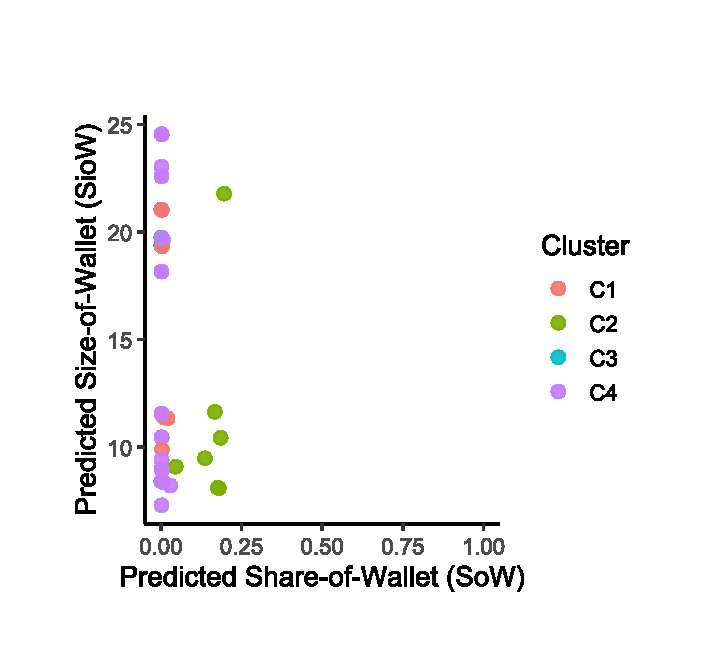
\includegraphics[width=0.75\textwidth]{figuras/sow-siow-k-means.pdf}
    \caption{Plano SoW--SioW para el conjunto de prueba. 
    Cada punto representa un cliente, coloreado según el clúster obtenido mediante \emph{k-means}. 
    El eje horizontal corresponde a la \emph{Share-of-Wallet} (SoW) predicha y el eje vertical a la 
    \emph{Size-of-Wallet} (SioW) predicha por el modelo \emph{pogit}.}
    \label{fig:sow_siow_kmeans}
\end{figure}


 \begin{figure}[H]
    \centering
    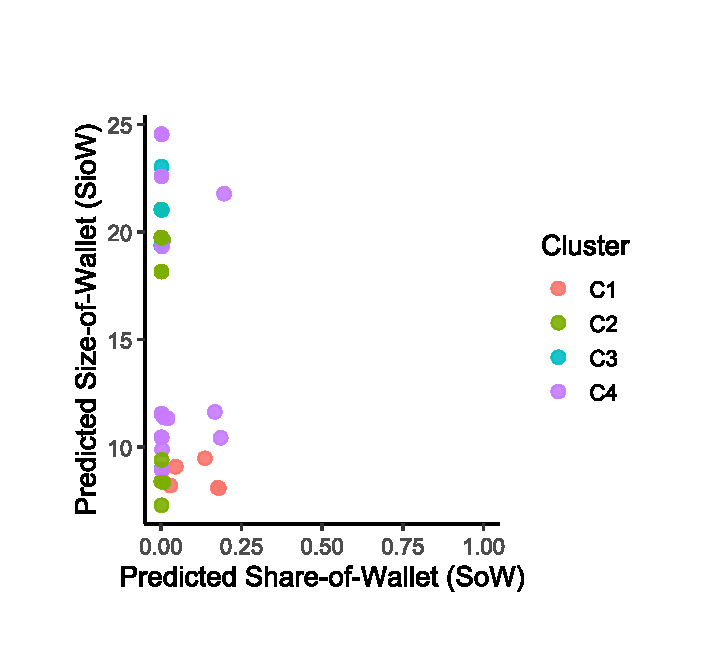
\includegraphics[width=0.75\textwidth]{figuras/sow-siow-k-mdd.pdf}
    \caption{Plano SoW--SioW para el conjunto de prueba. 
    Cada punto representa un cliente, coloreado según el clúster obtenido mediante \emph{k-medoids}. 
    El eje horizontal corresponde a la \emph{Share-of-Wallet} (SoW) predicha y el eje vertical a la 
    \emph{Size-of-Wallet} (SioW) predicha por el modelo \emph{pogit}.}
    \label{fig:sow_siow_kmedoids}
\end{figure}

    
    
        
    